% 国赛 (CUMCM) 2026 兼容模板

% 基于社区维护的 latexstudio/CUMCMThesis，并以全国组委会 2026 格式规范为准。

% 电子版提交使用 withoutpreface 去掉封面编号页，bwprint 黑白打印

\documentclass[withoutpreface,bwprint]{cumcmthesis}



% === 额外宏包 ===

\usepackage[framemethod=TikZ]{mdframed}

\usepackage[section]{placeins}

\usepackage{needspace}

\usepackage{algorithm2e}



% === 参考文献引用（数字型上标，配合 natbib）===

\usepackage[numbers,sort&compress]{natbib}



% === TikZ ===

\usetikzlibrary{arrows.meta,positioning,shapes.geometric,fit,calc}



% === 代码高亮设置 ===

\lstset{language=Python,basicstyle=\small\ttfamily,breaklines=true,frame=single,numbers=left,numberstyle=\tiny,extendedchars=true}



% === 摘要后排版修复 ===

\makeatletter

\renewenvironment{abstract}{%

  \if@twocolumn\section*{\abstractname}%

  \else\begin{center}{\zihao{3}\bfseries \abstractname\vspace{-.5em}\vspace{\z@}}\end{center}\quotation

  \fi}{\if@twocolumn\else\endquotation\newpage\fi}

\makeatother



\title{基于守恒型有限体积法与干基质量坐标的\\药材热风烘干耦合传热传质建模}



% MH-FLOAT-TUNE 受控浮动调参（防整页空白/一页一图）
% placeins 已由模板/cls 加载，此处不重复注入（避免 Option clash）
\renewcommand{\topfraction}{0.92}
\renewcommand{\bottomfraction}{0.9}
\renewcommand{\textfraction}{0.06}
\renewcommand{\floatpagefraction}{0.72}
\renewcommand{\dbltopfraction}{0.92}
\renewcommand{\dblfloatpagefraction}{0.72}
\setcounter{topnumber}{3}
\setcounter{bottomnumber}{2}
\setcounter{totalnumber}{4}
\begin{document}



\maketitle



% === 摘要（最后撰写）===

\begin{abstract}

药材热风烘干需兼顾干燥品质与能耗时长。本文以能量与水分质量守恒为起点，建立一维轴对称柱坐标
耦合传热传质模型，并构建统一的\textbf{守恒型有限体积}数值内核，以下四问在同一内核上逐层递进。

针对问题一，在附录2 常物性、恒定热风下调用上述内核求解预热阶段（$0\sim1800\,\mathrm{s}$）的
柱坐标耦合场，用后向 Euler 时间推进得到温度与含水率的时空分布；结果表明温度扰动尚未传到
轴心（轴心仅升至约 $33.6\,^{\circ}\mathrm{C}$），失水被限制在表面薄层，\textbf{轴心含水率仍保持初值 $2.55$}，
内部尚未进入干燥，该常物性解构成后续各问的\textbf{基准参照}。

针对问题二，改用附录3 温度—含水率变物性，令 $\rho,c_p,k,D$ 随场变化并在同一 Picard 回路内
联立更新，构成\textbf{双向强耦合}模型求解 $0\sim3\,\mathrm{h}$ 全过程；发现温度场全场温差已不足
$0.12\,^{\circ}\mathrm{C}$、近准稳态，而轴心含水率仅降到 $1.77$，据此揭示\textbf{传质比传热慢一到两个
数量级}（时间尺度比 $\tau_m/\tau_{\mathrm{th}}$ 由 $30$ 增至 $211$），为终点判据只建在含水率场上提供依据。

针对问题三，引入附件1 的时变热风边界，以轴心含水率的\textbf{首次穿越判据} $\max_r C<C_{\mathrm{th}}$
求解达标时长，并采用 Kirchhoff 积分平均处理界面扩散、避免调和平均被最小值锁死；算得
\textbf{达标时长 $t^{*}=57.262\,\mathrm{h}$}，传质毕奥数由约 $1.4$ 增至远大于 $1$，干燥由外部对流控制
转为内部扩散控制，解释了干燥曲线后段的拖尾。

针对问题四，进一步计入附件2 的体积收缩，借助干基质量不变量 $\rho_s R^2=\sigma$ 经 Landau 变换
把移动边界几何效应\textbf{凝聚为单一时变因子 $1/R(t)^2$} 并沿用同一内核求解；算得\textbf{达标时长
$t^{*}=50.898\,\mathrm{h}$}，较固定域基准缩短约 $11\%$，纯径向收缩假设经附件2 独立检验半径预测偏差
仅 $1.10\%$。全模型经 Bessel 解析解、Richardson 收敛阶与机器精度守恒审计验证，灵敏度分析
显示结果对环境外推稳健（$<0.6\%$），而忽略收缩会使 $t^*$ 虚高 $1.5$ 倍。

\keywords{耦合传热传质\quad 有限体积法\quad Kirchhoff 变换\quad 移动边界\quad 干基质量坐标}

\end{abstract}



% === 正文 ===

\label{mh:body-start}

\section{问题重述与分析}

\subsection{问题背景与任务}

药材热风烘干是把切成圆柱形的鲜药材置于恒定或时变的热风环境中，通过表面对流同时
带走热量与水分，使内部含水率逐步降到贮藏安全线的过程。药材可近似为半径
$R_0=2\,\mathrm{cm}$、长 $L=25\,\mathrm{cm}$ 的实心圆柱；因 $L\gg R_0$，端面效应可忽略，
热质输运沿径向占主导，问题退化为一维轴对称柱坐标下的耦合传热传质过程。初始温度
$T_0=28\,^{\circ}\mathrm{C}$、初始干基含水率 $C_0=2.55$，安全含水率阈值 $C_{\mathrm{th}}=0.15$。
题目给出三套物性附录（附录2 常物性、附录3 变物性、附录4 变物性且伴随体积收缩）与两份
实测附件（附件1 热风温度与空气含湿量时序、附件2 半径随时间的收缩数据），要求依次完成：

\begin{enumerate}
\item \textbf{问题一}，在附录2 常物性、恒定热风条件下，给出预热阶段（$0\sim1800\,\mathrm{s}$）
      药材内部温度场与含水率场的时空分布；
\item \textbf{问题二}，改用附录3 温度—含水率双向耦合的变物性，刻画 $0\sim3\,\mathrm{h}$ 内
      温度场与含水率场的全过程演化；
\item \textbf{问题三}，结合附件1 的时变热风，求内部各点含水率首次全部降至 $C_{\mathrm{th}}$
      以下所需的干燥时长；
\item \textbf{问题四}，进一步计入附件2 观测到的体积收缩，建立随时间缩小的移动边界模型，
      重新给出达标时长，并与问题三比较收缩的影响。
\end{enumerate}

\subsection{整体建模思路}

四问共享同一条守恒律骨架：由能量守恒与水分质量守恒，在柱坐标下得到一对以温度 $T$ 与
干基含水率 $C$ 为状态量的非稳态抛物型方程，表面施加 Robin 型对流换热与对流传质边界，
中心施加轴对称零通量条件\upcite{dincer2010,chaedir2019}。四问的差别只体现在\textbf{物性是否随场变化}、
\textbf{边界驱动是否时变}以及\textbf{求解域是否随时间收缩}三个层次的递进，因而适合"先建公共内核、
再逐问增量扩展"的组织方式：把守恒型离散格式、Kirchhoff 界面平均与时间推进统一放入公共章
（第\ref{sec:kernel}节），各问题章只描述本问新增或改变的部分。由于表面既是升温入口又是
失水出口，轴心因对称而通量为零、响应最慢，故"内部各点均达标"的判据必然由轴心含水率控制，
这一观察贯穿后两问的终点时刻计算。以下按题号分别说明各问的难点与建模路线。

\subsection{问题一的分析}

问题一在附录2 常物性、恒定热风下刻画预热阶段的耦合场。难点有二：一是柱坐标轴心处
散度算子含 $1/r$ 奇点，需要一种在轴心天然退化、不必人工正则化的离散方式；二是传热与
传质虽同为抛物型，却在此阶段呈现截然不同的推进深度。本问作为全篇基准，重点在于给出
温度场与含水率场的时空分布，并据此判断内部是否已进入实质干燥。

\subsection{问题二的分析}

问题二改用附录3 的温度—含水率变物性，$\rho,c_p,k,D$ 均随场演化，形成双向强耦合。
难点在于非线性物性与两个守恒方程的联立求解：温度经物性反过来影响扩散，含水率又改变
热容与导热。需在同一迭代回路内联立更新 $T$ 与 $C$，并辨识传热与传质的时间尺度差异，
为后续把终点判据只建立在含水率场上提供依据。

\subsection{问题三的分析}

问题三引入附件1 的时变热风边界，求内部各点含水率首次全部降至安全线以下的时长。
难点在于时变边界驱动下的首次穿越型终点判据，以及扩散系数随含水率跨越约一个数量级
所导致的界面平均失真——简单的算术或调和平均会显著偏离真实通量。需采用守恒型的界面
处理，才能避免干燥曲线后段出现非物理的拖尾。

\subsection{问题四的分析}

问题四进一步计入附件2 观测到的体积收缩，求解域随时间缩小，成为移动边界问题。难点在于
收缩带来的动网格困难与几何度规的时变。宜借助干物质总量守恒，把移动边界的几何效应
凝聚到固定计算域上的一个时变因子中，从而避免直接在收缩物理域上离散；同时须用观测数据
独立检验"纯径向收缩"这一关键假设，以免循环论证。


\section{模型假设}

结合题面已给条件，仅对题面未完全规定、而建模必须补足的现实简化作如下假设：

\begin{enumerate}
\item[(1)] \textbf{一维轴对称}。因 $L=25\,\mathrm{cm}\gg R_0=2\,\mathrm{cm}$，端面散失相对侧面
      可忽略，温度与含水率只沿半径 $r$ 变化，$\partial_\theta(\cdot)=\partial_z(\cdot)=0$。
      这使三维问题降为一维，保留了径向输运这一主导机制。
\item[(2)] \textbf{连续介质与局部平衡}。药材视为均质各向同性多孔介质，同一微元内固相、
      液态水与热量处于局部热力学平衡，可用单一温度 $T$ 与干基含水率 $C$ 描述其状态。
\item[(3)] \textbf{Fick 型扩散与 Fourier 型导热}。内部水分迁移服从以 $C$ 为势的 Fick 第二定律，
      热量传递服从 Fourier 定律；扩散系数 $D$ 与导热系数 $k$ 按各附录设定随 $C,T$ 变化。
\item[(4)] \textbf{对流型表面边界}。表面失水与散热速率正比于表面与热风之间的含水率差、温差，
      即 Robin 边界，传质、传热系数 $h_m,h$ 取为常数；这刻画了外部对流阻力的作用\upcite{giner2009}。
\item[(5)] \textbf{潜热不单列}。题面未给蒸发潜热 $L$，基准模型不显式扣除表面蒸发吸热，
      将其影响留待灵敏度分析定量评估（见第\ref{sec:sens}节），以避免引入未给定参数。
\item[(6)] \textbf{纯径向均匀收缩}（仅问题四）。附件2 的体积收缩按半径各向同性缩小处理，
      干物质总量守恒，收缩速率由附件2 数据经单调插值确定，不额外假设收缩动力学。
\end{enumerate}

\section{符号说明}

下表收录跨章节反复使用的核心符号，一次性下标与临时派生量在首次出现处就地说明。

\begin{center}
\small
\begin{longtable}{cll}
\toprule
符号 & 含义 & 单位 \\
\midrule
\endfirsthead
\toprule
符号 & 含义 & 单位 \\
\midrule
\endhead
\bottomrule
\endfoot
$r,\ t$ & 径向坐标、时间 & $\mathrm{m},\ \mathrm{s}$ \\
$R_0,\ R(t)$ & 初始半径、$t$ 时刻半径（问题四移动边界） & $\mathrm{m}$ \\
$T,\ T_{\mathrm{air}}$ & 药材温度、热风温度 & $^{\circ}\mathrm{C}$ \\
$C,\ C_{\mathrm{air}}$ & 干基含水率、空气等效含水率 & 1 \\
$C_0,\ C_{\mathrm{th}}$ & 初始含水率、安全含水率阈值 & 1 \\
$C_s,\ T_s$ & 表面含水率、表面温度 & 1,\ $^{\circ}\mathrm{C}$ \\
$\rho,\ c_p$ & 湿基密度、比热容 & $\mathrm{kg\,m^{-3}},\ \mathrm{J\,kg^{-1}K^{-1}}$ \\
$k$ & 导热系数 & $\mathrm{W\,m^{-1}K^{-1}}$ \\
$D$ & 水分扩散系数 & $\mathrm{m^2\,s^{-1}}$ \\
$h,\ h_m$ & 对流换热系数、对流传质系数 & $\mathrm{W\,m^{-2}K^{-1}},\ \mathrm{m\,s^{-1}}$ \\
$T_K$ & 绝对温度 $T+273.15$ & $\mathrm{K}$ \\
$\alpha$ & 热扩散率 $k/(\rho c_p)$ & $\mathrm{m^2\,s^{-1}}$ \\
$\mathrm{Bi}_m$ & 传质毕奥数 $h_m R_0/D$ & 1 \\
$\Phi(C)$ & 扩散系数的 Kirchhoff 积分势 & $\mathrm{m^2\,s^{-1}}$ \\
$\xi$ & 固定域无量纲坐标 $r/R(t)$ & 1 \\
$\sigma$ & 干基质量不变量 $\rho_s R^2$ & $\mathrm{kg\,m^{-1}}$ \\
$w_j$ & 控制体柱坐标测度权 & 1 \\
$t^{*}$ & 内部各点首次全部达标的时刻 & $\mathrm{h}$ \\
\end{longtable}
\end{center}


\section{公共建模内核：守恒型柱坐标耦合场的有限体积求解}\label{sec:kernel}

四个子问题共享同一套守恒律、离散格式与时间推进策略。本节一次性建立这一公共内核，
后续问题章只在此基础上说明"保留了什么、新增了什么、结果如何改变"，不再重复整套推导。
四问在同一内核上的递进关系与总体技术路线见图~\ref{fig:roadmap}。

\begin{figure}[H]
  \centering
  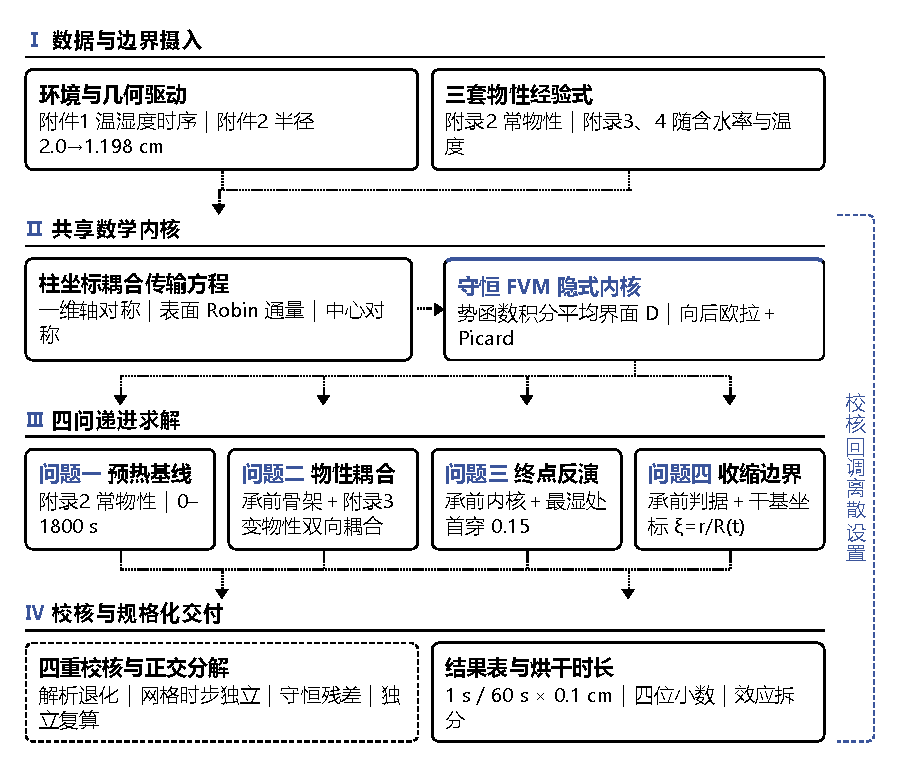
\includegraphics[width=0.94\textwidth,height=0.8\textheight,keepaspectratio]{../figures/fig_roadmap.pdf}
  \caption{总体技术路线：从守恒律到公共数值内核，再逐问增量扩展}
  \label{fig:roadmap}
\end{figure}

图~\ref{fig:roadmap} 表明四问并非彼此独立的四个模型，而是同一守恒型有限体积内核在
"物性—边界—求解域"三个层次上的递进，故各问题章只描述本问新增或改变的部分。

\subsection{控制方程与定解条件}

以柱坐标轴心为原点，取半径 $r\in[0,R_0]$。对任意以轴为中心、半径 $r$ 的同轴圆柱控制面，
能量守恒与水分质量守恒给出通量的散度形式；在轴对称、忽略轴向与周向输运后，得到一对
非稳态抛物型方程：
\begin{equation}\label{eq:pde}
\rho c_p\,\frac{\partial T}{\partial t}=\frac{1}{r}\frac{\partial}{\partial r}\!\left(r\,k\,\frac{\partial T}{\partial r}\right),
\qquad
\frac{\partial C}{\partial t}=\frac{1}{r}\frac{\partial}{\partial r}\!\left(r\,D\,\frac{\partial C}{\partial r}\right),
\qquad 0<r<R_0 .
\end{equation}
式~\eqref{eq:pde} 中左端为单位体积的热/水分储量变化率，右端 $\frac{1}{r}\partial_r(r\,\cdot)$ 是柱坐标下的
散度算子，$k,D$ 分别为导热系数与水分扩散系数。表面 $r=R_0$ 处，内部扩散/导热通量必须与
外部对流带走的水分/热量平衡，得 Robin 边界；轴心 $r=0$ 处由对称性得零通量：
\begin{equation}\label{eq:bc}
\left.-D\frac{\partial C}{\partial r}\right|_{R_0}=h_m\,(C_s-C_{\mathrm{air}}),\quad
\left.-k\frac{\partial T}{\partial r}\right|_{R_0}=h\,(T_s-T_{\mathrm{air}}),\quad
\left.\frac{\partial C}{\partial r}\right|_{0}=\left.\frac{\partial T}{\partial r}\right|_{0}=0 .
\end{equation}
初始条件为 $T(r,0)=T_0=28\,^{\circ}\mathrm{C}$、$C(r,0)=C_0=2.55$。几何与边界条件的对应关系见
图~\ref{fig:tikz_geometry_bc}。

\begin{figure}[H]
  \centering
  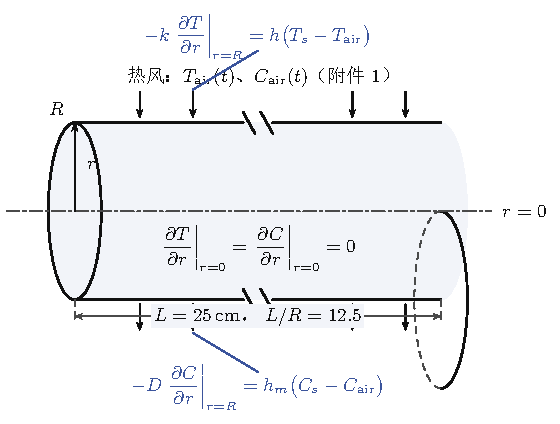
\includegraphics[width=0.9\textwidth,height=0.8\textheight,keepaspectratio]{../figures/tikz_geometry_bc.pdf}
  \caption{圆柱几何与柱坐标边界条件：表面 Robin、轴心零通量、端面忽略}
  \label{fig:tikz_geometry_bc}
\end{figure}

图~\ref{fig:tikz_geometry_bc} 明确了三类边界的物理归属：表面同时承担对流换热与对流传质，
轴心因对称退化为绝热绝湿面，端面则因长径比大而被忽略。式~\eqref{eq:pde}--\eqref{eq:bc}
是四问共用的连续模型，各问的差异仅在于 $\rho,c_p,k,D$ 与 $T_{\mathrm{air}},C_{\mathrm{air}}$ 的具体形式。
热量与水分的输运路径见图~\ref{fig:scene}。

\begin{figure}[H]
  \centering
  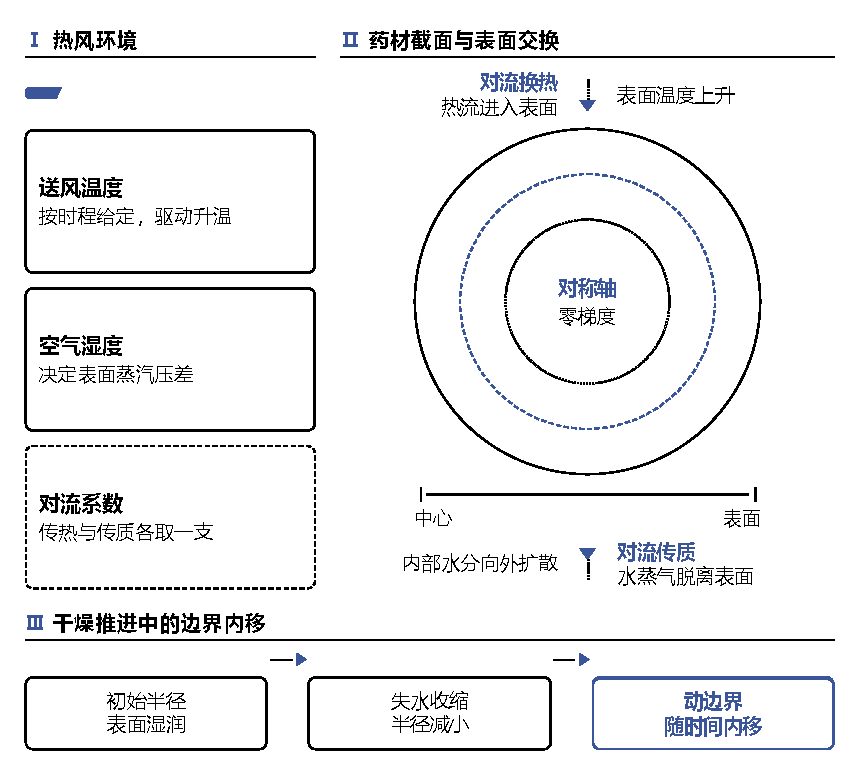
\includegraphics[width=0.92\textwidth,height=0.8\textheight,keepaspectratio]{../figures/fig_scene.pdf}
  \caption{热风烘干中的表面对流换热、对流传质与内部径向扩散}
  \label{fig:scene}
\end{figure}

图~\ref{fig:scene} 表明：热风以对流换热系数 $h$ 向表面供热，水分以对流传质系数 $h_m$
从表面逸出，内部则由导热与扩散把边界扰动向轴心传播；轴心响应最慢，是"内部各点均达标"
判据的控制点。

\subsection{三套物性与扩散系数的量级差异}

三套附录给出的物性形式不同：附录2 为常物性；附录3、附录4 均取
$\rho=\rho_0+\rho_1 C$、$c_p=c_{p0}+c_{p1}\frac{C}{C+1}$、$k=k_0+k_1\frac{C}{C+1}$，扩散系数则统一采用
Arrhenius 型
\begin{equation}\label{eq:diff}
D(C,T)=D_0\,\exp\!\left(-\frac{a}{C}\right)\exp\!\left(-\frac{E}{T_K}\right),\qquad T_K=T+273.15 ,
\end{equation}
其中 $\exp(-a/C)$ 刻画低含水率时自由水减少导致的扩散受阻，$\exp(-E/T_K)$ 为温度激活项，
$E=3850\,\mathrm{K}$\upcite{tong1990,ma2026}。附录3 取 $D_0=2.4\times10^{-3},a=0.45$，附录4 取
$D_0=4.2\times10^{-4},a=0.30$，各附录完整物性见表~\ref{tab:properties}。三套扩散系数的量级
对比与附录3 的二维响应面见图~\ref{fig:diffusivity_range} 与图~\ref{fig:diffusivity_contour}。

% 表：三套附录物性模型与关键参数
% 数据来源：PROBLEM_FACTS.json → code/params.py（OCR SHA256 核验）
\begin{table}[H]
  \centering
  \caption{三套附录物性模型对照}
  \label{tab:properties}
  \small
  \begin{tabular}{llll}
    \toprule
    物性量 & 附录2（问题1） & 附录3（问题2、3） & 附录4（问题4） \\
    \midrule
    密度 $\rho$ / (kg$\cdot$m$^{-3}$)
      & $820$
      & $650+128\,C$
      & $760+90\,C$ \\
    比热 $c_p$ / (J$\cdot$kg$^{-1}$K$^{-1}$)
      & $2600$
      & $1450+2736\dfrac{C}{C+1}$
      & $1850+2150\dfrac{C}{C+1}$ \\
    导热 $k$ / (W$\cdot$m$^{-1}$K$^{-1}$)
      & $0.36$
      & $0.21+0.38\dfrac{C}{C+1}$
      & $0.12+0.20\dfrac{C}{C+1}$ \\
    扩散系数 $D$ / (m$^2\cdot$s$^{-1}$)
      & $7{\times}10^{-9}e^{-0.89/C}$
      & $2.4{\times}10^{-3}e^{-0.45/C}e^{-3850/T_K}$
      & $4.2{\times}10^{-4}e^{-0.30/C}e^{-3850/T_K}$ \\
    \midrule
    $D$ 初始值（$C_0$，$28^\circ$C）
      & $4.938{\times}10^{-9}$
      & $5.642{\times}10^{-9}$
      & 随工况 \\
    $D$ 终点值（$C_{\rm th}$，$50^\circ$C）
      & ---
      & $8.001{\times}10^{-10}$
      & 随工况 \\
    温度依赖性
      & 无
      & Arrhenius
      & Arrhenius \\
    边界域
      & 固定 $R_0$
      & 固定 $R_0$
      & 动边界 $R(t)$ \\
    \bottomrule
  \end{tabular}

  \vspace{2pt}
  \parbox{0.94\linewidth}{\footnotesize
  注：$C$ 为干基含水率（kg$\cdot$kg$^{-1}$），$T_K$ 为开尔文温度。
  共用参数：$R_0=2$ cm，$L=25$ cm，$T_0=28^\circ$C，$C_0=2.55$，达标阈值
  $C_{\rm th}=0.15$，对流换热 $h=25$ W$\cdot$m$^{-2}$K$^{-1}$，
  对流传质 $h_m=8{\times}10^{-7}$ m$\cdot$s$^{-1}$。
  $D$ 锚点值由上式复算，与题面校核点一致。}
\end{table}


表~\ref{tab:properties} 给出的锚点表明：初始状态 $D(C_0,28\,^{\circ}\mathrm{C})$ 在附录2、附录3
分别为 $4.938\times10^{-9}$ 与 $5.642\times10^{-9}\,\mathrm{m^2/s}$，量级相当；但降到阈值附近
$D(C_{\mathrm{th}},50\,^{\circ}\mathrm{C})$ 骤降至 $8.001\times10^{-10}$，说明干燥末期扩散显著变慢，这正是
干燥曲线后段拖尾的根源。

\begin{figure}[H]
  \centering
  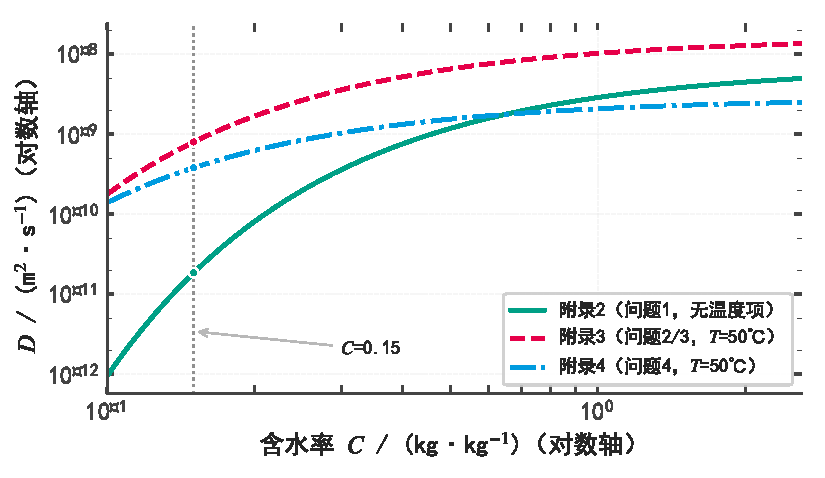
\includegraphics[width=0.9\textwidth,height=0.8\textheight,keepaspectratio]{../figures/fig_diffusivity_range.pdf}
  \caption{三套附录扩散系数在 $C\in[C_{\mathrm{th}},C_0]$ 上的量级对比}
  \label{fig:diffusivity_range}
\end{figure}

图~\ref{fig:diffusivity_range} 显示，随含水率从 $C_0$ 降到 $C_{\mathrm{th}}$，扩散系数跨越约一个数量级，
且三套物性的下降斜率因 $a$ 不同而分化：$a$ 越大（附录2 的等效 $a=0.89$），末期抑制越强。
这一强非线性使得直接对 $D\partial_r C$ 作简单平均会显著失真，必须在离散时对界面扩散通量
作专门处理，详见 \ref{sub:kirchhoff} 节。

\begin{figure}[H]
  \centering
  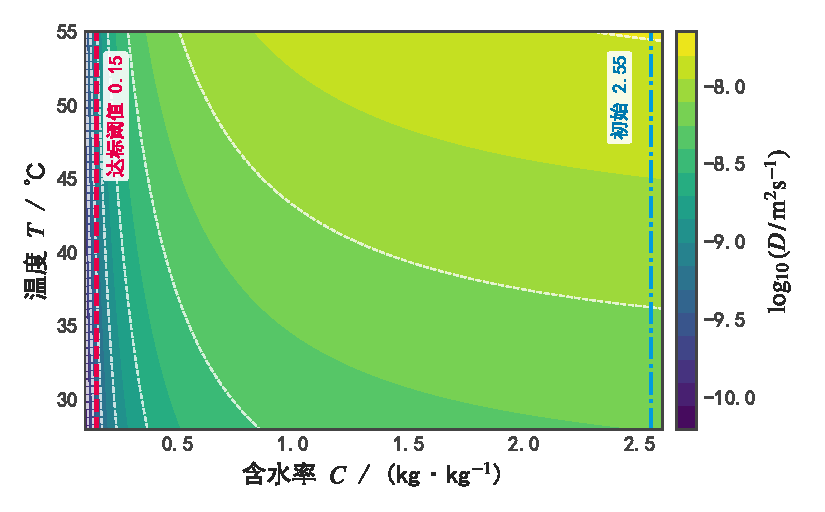
\includegraphics[width=0.9\textwidth,height=0.8\textheight,keepaspectratio]{../figures/fig_diffusivity_contour.pdf}
  \caption{附录3 扩散系数 $D(C,T)$ 在含水率—温度平面上的二维响应面}
  \label{fig:diffusivity_contour}
\end{figure}

图~\ref{fig:diffusivity_contour} 进一步表明 $D$ 对 $C$ 的敏感度远高于对 $T$：等值线沿含水率
方向密集、沿温度方向平缓，说明在本题温区（$28\sim50\,^{\circ}\mathrm{C}$）内，含水率是控制扩散的
主因，温度主要通过 Arrhenius 项作二阶调节。这为问题三、四把终点判据建立在含水率场上
（而非温度场）提供了依据。

\subsection{守恒型有限体积离散}

把 $[0,R_0]$ 划分为 $N$ 个控制体，节点 $r_j$ 位于控制体形心，控制面位于 $r_{j\pm1/2}$。
对式~\eqref{eq:pde} 在第 $j$ 个环形控制体上作体积分，利用散度定理把体积分化为控制面上的
通量差，得到严格守恒的半离散格式（以 $C$ 为例，$T$ 同构）：
\begin{equation}\label{eq:fvm}
w_j\,\frac{\mathrm{d}C_j}{\mathrm{d}t}
=\frac{2}{R_0^2}\Big[\,r_{j+\frac12}\,\widehat{D}_{j+\frac12}\,\frac{C_{j+1}-C_j}{\Delta r}
-\,r_{j-\frac12}\,\widehat{D}_{j-\frac12}\,\frac{C_j-C_{j-1}}{\Delta r}\,\Big],
\qquad
w_j=\xi_{j+\frac12}^2-\xi_{j-\frac12}^2 ,
\end{equation}
其中 $\xi=r/R_0$，柱坐标测度权 $w_j$ 满足 $\sum_j w_j=1$（等价于 $\sum_j w_j-\pi R_0^2$ 归零，
见表~\ref{tab:verification}）。式~\eqref{eq:fvm} 的关键在于：\textbf{最内控制体的内侧控制面
面积 $r_{1/2}\to0$ 结构性地为零}，因而轴心奇点 $1/r$ 被离散格式天然消去，无需对
$\frac{1}{r}\partial_r$ 作洛必达展开或人工正则化。网格与控制体通量平衡见图~\ref{fig:tikz_fvm_mesh}。

\begin{figure}[H]
  \centering
  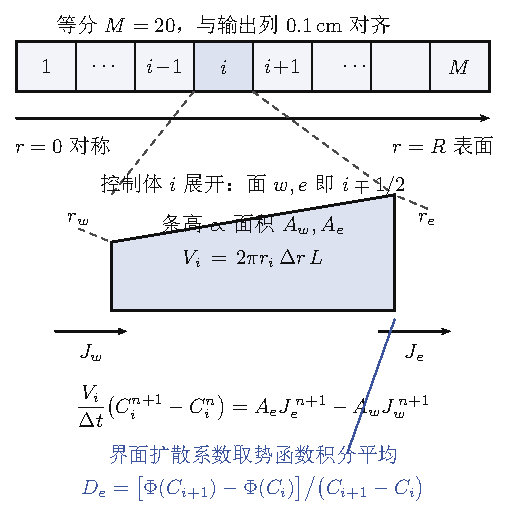
\includegraphics[width=0.8\textwidth,height=0.8\textheight,keepaspectratio]{../figures/tikz_fvm_mesh.pdf}
  \caption{有限体积网格：节点、控制面与环形控制体上的进出通量平衡}
  \label{fig:tikz_fvm_mesh}
\end{figure}

图~\ref{fig:tikz_fvm_mesh} 显示每个控制体的净储量变化等于其两侧控制面的通量差，逐控制体
求和后内部通量成对抵消，只剩表面对流项，从而在离散层面精确复现连续守恒律。这一守恒性
在第\ref{sec:verify}节被量化为 $10^{-13}\sim10^{-16}$ 量级的机器精度残差。

\subsection{界面扩散系数的 Kirchhoff 积分平均}\label{sub:kirchhoff}

式~\eqref{eq:fvm} 需要控制面处的等效扩散系数 $\widehat{D}_{j\pm1/2}$。由于 $D(C)$ 随 $C$ 跨越
约一个数量级（图~\ref{fig:diffusivity_range}），常用的算术平均会高估、调和平均会被最小值
锁死。为在界面处保持通量 $D\,\partial_r C=\partial_r\Phi(C)$ 的一致性，引入 Kirchhoff 势
$\Phi(C)=\int^{C} D(s)\,\mathrm{d}s$\upcite{gama2021,ramos2024}。对 Arrhenius 型
式~\eqref{eq:diff} 的含水率因子解析积分得
\begin{equation}\label{eq:kirchhoff}
\Phi(C)=C\,e^{-a/C}-a\,E_1\!\left(\frac{a}{C}\right),\qquad
\widehat{D}_{j+\frac12}=\frac{\Phi(C_{j+1})-\Phi(C_j)}{C_{j+1}-C_j},
\end{equation}
其中 $E_1(\cdot)$ 为指数积分函数，数值上按其标准级数与渐近展开求值。式~\eqref{eq:kirchhoff}
的界面平均保证了跨界面扩散通量守恒，其对达标时刻的影响见图~\ref{fig:interface_scheme}
与第\ref{sec:sens}节：改用算术平均仅使 $t^*$ 变化 $-1.80\%$，而调和平均因被
最小值锁死产生 $557.76\,\mathrm{h}$ 的非物理结果。

\begin{figure}[H]
  \centering
  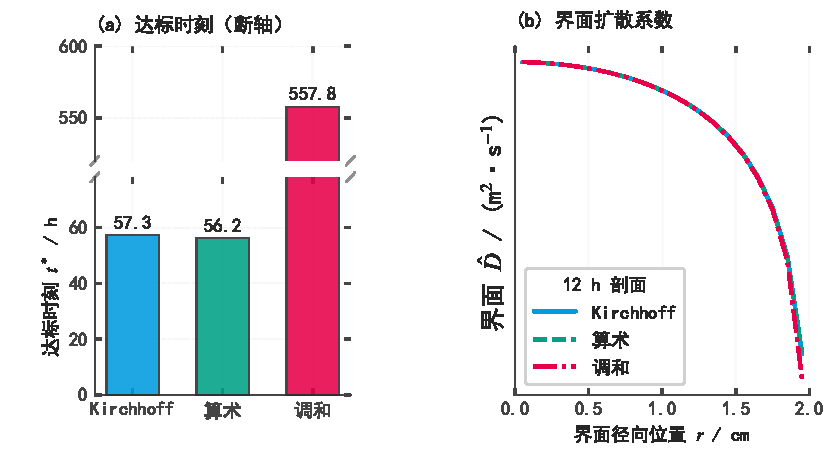
\includegraphics[width=0.9\textwidth,height=0.8\textheight,keepaspectratio]{../figures/fig_interface_scheme.pdf}
  \caption{界面扩散系数平均方式（Kirchhoff、算术、调和）对达标时刻的影响}
  \label{fig:interface_scheme}
\end{figure}

图~\ref{fig:interface_scheme} 直观显示调和平均在 $D$ 跨量级处严重偏离，而 Kirchhoff 积分平均
与算术平均接近且更符合通量守恒，故全文界面扩散系数统一采用式~\eqref{eq:kirchhoff}。

\subsection{时间推进：后向 Euler 与 Picard 内迭代}

物性 $\rho,c_p,k,D$ 依赖待求的 $T,C$，式~\eqref{eq:fvm} 是强非线性刚性方程组。为兼顾稳定性
与守恒性，采用 $L$-稳定的后向 Euler 格式（$\theta=1$），并在每个时间步用 Picard 迭代把
非线性物性冻结更新\upcite{blasik2015}：
\begin{equation}\label{eq:picard}
\frac{\mathbf{U}^{n+1,(m+1)}-\mathbf{U}^{n}}{\Delta t}
=\mathcal{L}\!\big(\mathbf{U}^{n+1,(m)}\big)\,\mathbf{U}^{n+1,(m+1)},
\qquad
\big\|\mathbf{U}^{(m+1)}-\mathbf{U}^{(m)}\big\|_\infty<\varepsilon ,
\end{equation}
其中 $\mathbf{U}=(T,C)$ 在\textbf{同一}迭代回路内联立更新以保持双向耦合，$\mathcal{L}$ 为
按上一迭代场组装的三对角算子，收敛容差 $\varepsilon=10^{-11}$、最大迭代 40 次。实测每步
Picard 残差降至 $9.998\times10^{-12}$（表~\ref{tab:verification}）。此外，Arrhenius 项在
Kelvin 下计算并施加 $200<T_K<500$ 的物理性断言，避免温度越界导致的数值发散。

至此，公共内核（守恒律—有限体积—Kirchhoff 界面—后向 Euler/Picard）建立完毕。以下四章
分别说明各问在此内核上的具体设定与结果。


\section{问题一：常物性柱坐标耦合场的预热阶段温度与水分分布}\label{sec:p1}

\subsection{本问设定与建模}

问题一采用附录2 常物性、恒定热风（$T_{\mathrm{air}}=50\,^{\circ}\mathrm{C}$），求预热阶段
$0\sim1800\,\mathrm{s}$ 内的温度场与含水率场。此时式~\eqref{eq:pde} 的系数 $\rho,c_p,k,D$ 均为常数，
方程退化为经典的柱坐标线性热扩散/物质扩散对，热扩散率 $\alpha=k/(\rho c_p)=1.6886\times10^{-7}\,\mathrm{m^2/s}$，
对应特征热时间 $\tau_{\mathrm{th}}=R_0^2/\alpha\approx2368.9\,\mathrm{s}$。求解直接调用公共内核
（式~\eqref{eq:fvm}--\eqref{eq:picard}），因常物性故 Picard 迭代一步即收敛。

\subsection{结果与分析}

图~\ref{fig:field_heatmap_p1} 给出温度场与含水率场在 $(r,t)$ 平面上的时空演化。

\begin{figure}[H]
  \centering
  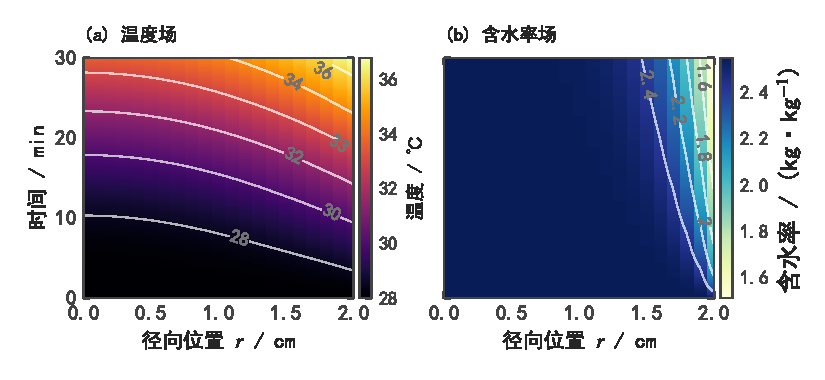
\includegraphics[width=0.9\textwidth,height=0.8\textheight,keepaspectratio]{../figures/fig_field_heatmap_p1.pdf}
  \caption{问题1 温度场（左）与含水率场（右）在预热阶段的时空演化}
  \label{fig:field_heatmap_p1}
\end{figure}

由图~\ref{fig:field_heatmap_p1} 可见，温度扰动自表面向轴心推进，$1800\,\mathrm{s}$ 时轴心温度
仅由 $28\,^{\circ}\mathrm{C}$ 升到约 $33.6\,^{\circ}\mathrm{C}$，尚未达到热风温度，印证预热阶段的特征时间
$\tau_{\mathrm{th}}\approx2369\,\mathrm{s}$ 与观测时窗相当、升温未完成。含水率场则几乎只在近表面
薄层内下降，轴心含水率仍保持在 $C_0=2.55$。径向剖面见图~\ref{fig:radial_profiles}。

\begin{figure}[H]
  \centering
  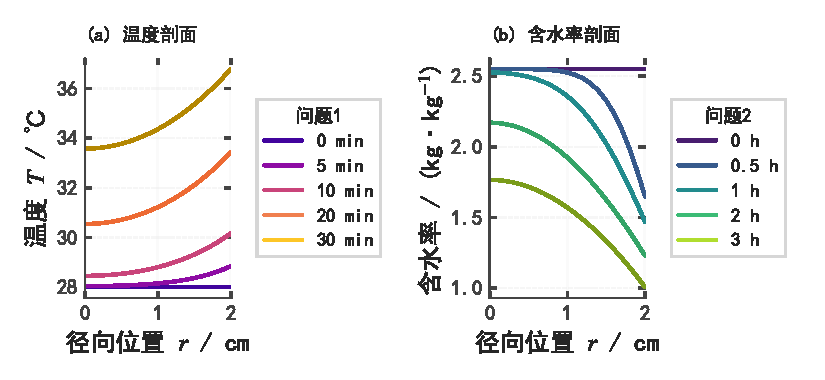
\includegraphics[width=0.9\textwidth,height=0.8\textheight,keepaspectratio]{../figures/fig_radial_profiles.pdf}
  \caption{问题1 不同时刻温度剖面（左）与问题2 含水率剖面（右）的径向分布}
  \label{fig:radial_profiles}
\end{figure}

图~\ref{fig:radial_profiles} 左侧的温度剖面显示 $1800\,\mathrm{s}$ 时沿半径由轴心到表面为
$33.58$,\allowbreak\,$33.77$,\allowbreak\,$34.37$,\allowbreak\,$35.36$,\allowbreak\,$36.79\,^{\circ}\mathrm{C}$，呈单调升高的边界层型分布；对应含水率由轴心
到表面为 $2.5500$,\allowbreak\,$2.5496$,\allowbreak\,$2.5376$,\allowbreak\,$2.3763$,\allowbreak\,$1.5125$，即\textbf{只有最外一到两层含水率明显下降，
轴心几乎未失水}。这说明预热阶段传质被限制在表面薄层，内部尚未"感知"到干燥，也解释了
为何该阶段不宜用于反演内部含水率——内部信息尚未从边界传入。问题一的结果构成后续变物性、
时变边界与移动边界模型的基准解，各问最终数值汇总见表~\ref{tab:main_results}。


\section{问题二：变物性双向强耦合下的全过程温度与水分场}\label{sec:p2}

\subsection{相对问题一的增量：变物性与双向耦合}

问题二保留问题一的柱坐标控制方程~\eqref{eq:pde} 与恒定热风，但把附录2 常物性替换为附录3
变物性：$\rho=650+128C$、$c_p=1450+2736\frac{C}{C+1}$、$k=0.21+0.38\frac{C}{C+1}$，扩散系数按
式~\eqref{eq:diff} 取 $D_0=2.4\times10^{-3},a=0.45$。此时含水率 $C$ 通过 $\rho,c_p,k$ 影响温度场，
温度 $T$ 又通过 Arrhenius 项 $\exp(-E/T_K)$ 影响扩散、进而改变含水率，构成\textbf{双向强耦合}。
求解时 $T,C$ 在同一 Picard 回路内联立更新（式~\eqref{eq:picard}），观测时窗取 $0\sim3\,\mathrm{h}$。

\subsection{结果与分析}

图~\ref{fig:field_heatmap_p2} 给出含水率场的时空演化与边缘剖面。

\begin{figure}[H]
  \centering
  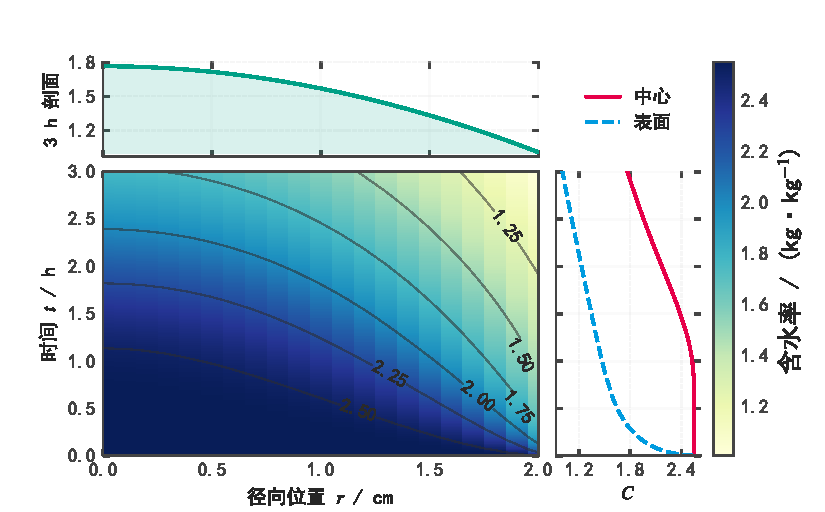
\includegraphics[width=0.9\textwidth,height=0.8\textheight,keepaspectratio]{../figures/fig_field_heatmap_p2.pdf}
  \caption{问题2 含水率场时空演化与不同时刻的边缘剖面}
  \label{fig:field_heatmap_p2}
\end{figure}

由图~\ref{fig:field_heatmap_p2}，$3\,\mathrm{h}$ 时轴心含水率降至 $1.7662$、表面降至 $1.0078$，
沿半径由轴心到表面为 $1.7662$,\allowbreak\,$1.7165$,\allowbreak\,$1.5701$,\allowbreak\,$1.3331$,\allowbreak\,$1.0078$（对应问题2 剖面见
图~\ref{fig:radial_profiles} 右）；与问题一相比，失水已从表面薄层推进到全径，但\textbf{距阈值
$0.15$ 仍有量级差距}，说明 $3\,\mathrm{h}$ 远未达标，为问题三的长时程计算埋下伏笔。温度场
等值线见图~\ref{fig:temp_contour_p2}。

\begin{figure}[H]
  \centering
  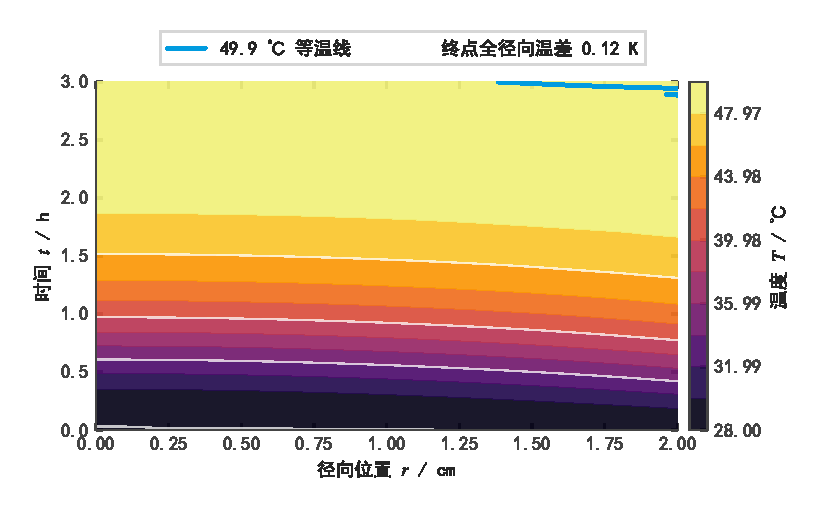
\includegraphics[width=0.9\textwidth,height=0.8\textheight,keepaspectratio]{../figures/fig_temp_contour_p2.pdf}
  \caption{问题2 温度场等值线与 $49.9\,^{\circ}\mathrm{C}$ 等温线}
  \label{fig:temp_contour_p2}
\end{figure}

图~\ref{fig:temp_contour_p2} 显示 $3\,\mathrm{h}$ 时温度场已近乎均匀：沿半径为
$49.8495$,\allowbreak\,$49.8554$,\allowbreak\,$49.8746$,\allowbreak\,$49.9101$,\allowbreak\,$49.9664\,^{\circ}\mathrm{C}$，全场温差不足 $0.12\,^{\circ}\mathrm{C}$，
$49.9\,^{\circ}\mathrm{C}$ 等温线已逼近轴心，表明\textbf{温度场早已进入准稳态，而含水率场仍在缓慢演化}。
这一"热快质慢"的分离是本题的核心机理，定量刻画见图~\ref{fig:timescale_split}。

\begin{figure}[H]
  \centering
  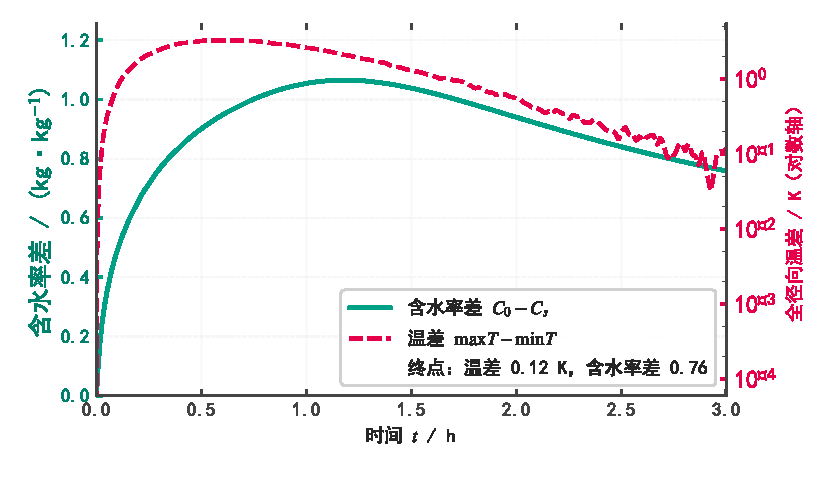
\includegraphics[width=0.9\textwidth,height=0.8\textheight,keepaspectratio]{../figures/fig_timescale_split.pdf}
  \caption{问题2 传热与传质特征时间尺度的分离}
  \label{fig:timescale_split}
\end{figure}

图~\ref{fig:timescale_split} 比较传热与传质的特征时间：传质时间与传热时间之比
$\tau_m/\tau_{\mathrm{th}}$ 由初始约 $30$ 增大到终点约 $211$，即水分迁移比热量传递慢一到两个数量级，
且随含水率下降差距进一步拉大。这解释了为何可以近似认为温度场先达稳态、再驱动缓慢的
失水过程，也为问题三只在含水率场上设终点判据（而非温度场）提供了尺度依据。


\section{问题三：基于首次穿越判据的长时程干燥终点时长反演}\label{sec:p3}

\subsection{相对问题二的增量：时变边界与终点判据}

问题三在问题二（附录3 变物性）基础上把恒定热风替换为附件1 实测的时变热风温度
$T_{\mathrm{air}}(t)$ 与空气含湿量 $C_{\mathrm{air}}(t)$，并求内部各点含水率首次全部降到阈值以下的
时长。附件1、附件2 的统计特征见表~\ref{tab:data_stats}，时序驱动见图~\ref{fig:env_driving}。

% 表：附件输入数据描述性统计
% 数据来源：user_data/附件1.xlsx（241 行）、user_data/附件2.xlsx（145 行）
\begin{table}[H]
  \centering
  \caption{附件输入数据描述性统计}
  \label{tab:data_stats}
  \small
  \begin{tabular}{llrrrrrr}
    \toprule
    来源 & 变量（单位） & 样本数 & 最小值 & 最大值 & 均值 & 中位数 & 标准差 \\
    \midrule
    附件1 & 时间（s）                          & 241 & 0      & 14400  & 7200   & 7200   & 4182.894 \\
    附件1 & 热风温度（$^\circ$C）              & 241 & 28.000 & 50.246 & 47.245 & 49.757 & 5.115 \\
    附件1 & 空气水分浓度（kg$\cdot$kg$^{-1}$）  & 241 & 0.0196 & 0.0503 & 0.0448 & 0.0491 & 0.0081 \\
    \midrule
    附件2 & 时间（s）                          & 145 & 0      & 259200 & 129600 & 129600 & 75603.571 \\
    附件2 & 药材半径（cm）                     & 145 & 1.198  & 2.000  & 1.246  & 1.200  & 0.127 \\
    \bottomrule
  \end{tabular}

  \vspace{2pt}
  \parbox{0.92\linewidth}{\footnotesize
  注：标准差为样本标准差（$n-1$ 自由度）。两附件时间列均为等距采样
  （附件1 步长 60 s，附件2 步长 1800 s），故均值与中位数重合。
  半径均值 1.246 cm 高于中位数 1.200 cm，反映收缩集中在早期、随后进入平台。}
\end{table}


\begin{figure}[H]
  \centering
  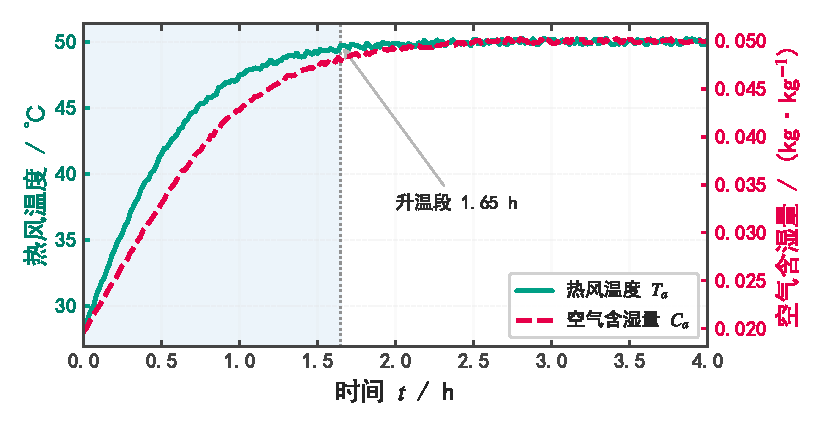
\includegraphics[width=0.9\textwidth,height=0.8\textheight,keepaspectratio]{../figures/fig_env_driving.pdf}
  \caption{附件1 热风温度与空气含湿量的双轴时序（模型的时变边界驱动）}
  \label{fig:env_driving}
\end{figure}

图~\ref{fig:env_driving} 与表~\ref{tab:data_stats} 显示，热风温度在约 $0.5\,\mathrm{h}$ 内由
$28\,^{\circ}\mathrm{C}$ 升至并稳定在 $50\,^{\circ}\mathrm{C}$ 附近（均值 $47.2\,^{\circ}\mathrm{C}$），空气含湿量
均值约 $0.045$；附件1 仅覆盖前 $4\,\mathrm{h}$，而达标需数十小时，故对 $t>4\,\mathrm{h}$ 采用
"保持末值"作为基准外推，其影响在第\ref{sec:sens}节量化（不足 $0.6\%$）。由于内部各点中
\textbf{轴心含水率最高、下降最慢}（图~\ref{fig:field_heatmap_p1}、\ref{fig:field_heatmap_p2} 已示），
"内部各点均达标"等价于轴心达标，故终点时刻取首次穿越
\begin{equation}\label{eq:endpoint}
t^{*}=\inf\Big\{t:\ \max_{0\le r\le R_0}C(r,t)<C_{\mathrm{th}}\Big\}
     =\inf\Big\{t:\ C(0,t)<C_{\mathrm{th}}\Big\},
\end{equation}
并在跨越阈值的相邻两输出步之间对 $C(0,t)$ 作线性插值定位 $t^*$，避免受输出步长限制。

\subsection{结果与分析}

图~\ref{fig:drying_curve} 给出中心与表面含水率的干燥曲线及阈值首次穿越。

\begin{figure}[H]
  \centering
  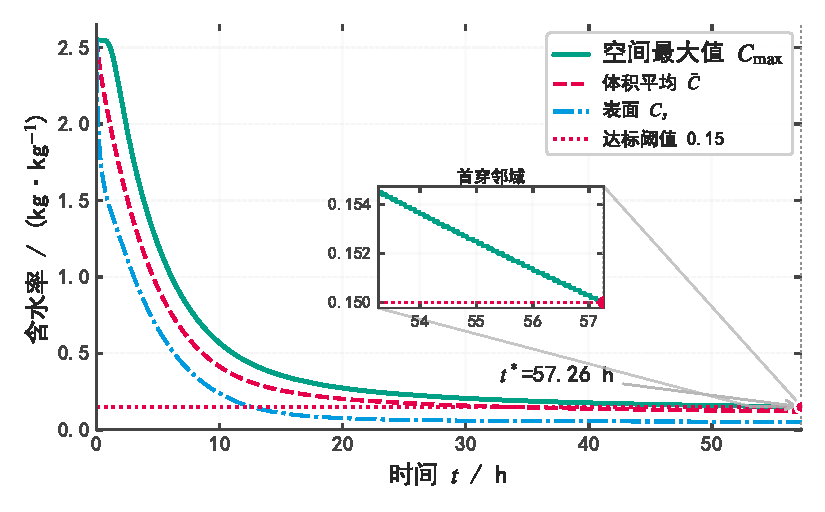
\includegraphics[width=0.9\textwidth,height=0.8\textheight,keepaspectratio]{../figures/fig_drying_curve.pdf}
  \caption{问题3 中心/表面含水率干燥曲线与达标阈值 $C_{\mathrm{th}}=0.15$ 的首次穿越}
  \label{fig:drying_curve}
\end{figure}

\begin{sloppypar}
由图~\ref{fig:drying_curve}，轴心含水率在 $t^{*}=57.262\,\mathrm{h}$ 首次降到
$C_{\mathrm{th}}=0.15$（此刻 $\max_r C=0.14999515$，前一输出步为 $0.15001272$），此时表面已降至
$0.0525$，与空气等效含水率 $C_{\mathrm{air}}\approx0.0499$ 接近但未越过，表面失水趋于平衡。
干燥曲线呈典型的\textbf{先快后慢}：初期近表面陡降，末期因 $D$ 随 $C$ 减小而拖尾。各时刻
径向剖面的堆叠演化见图~\ref{fig:ridgeline_profile}。
\end{sloppypar}

\begin{figure}[H]
  \centering
  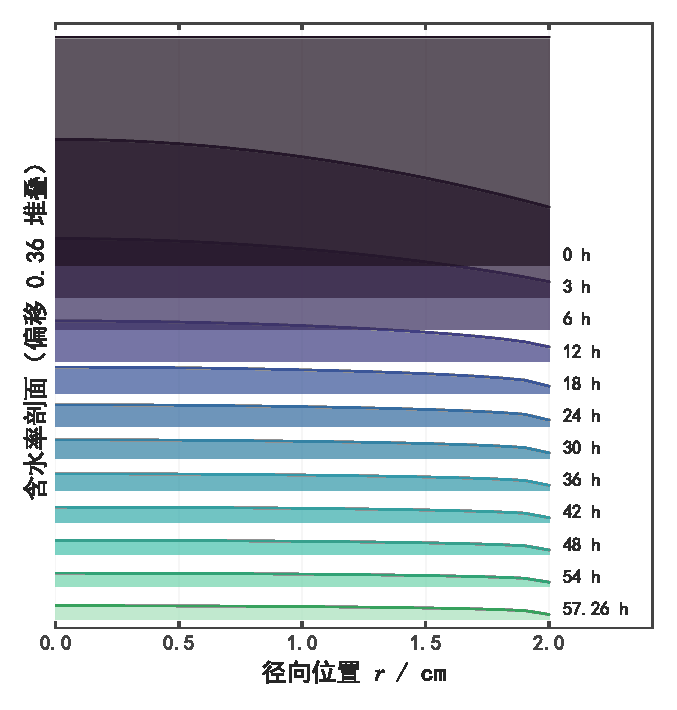
\includegraphics[width=0.8\textwidth,height=0.8\textheight,keepaspectratio]{../figures/fig_ridgeline_profile.pdf}
  \caption{问题3 各时刻径向含水率剖面的堆叠（ridgeline）演化}
  \label{fig:ridgeline_profile}
\end{figure}

图~\ref{fig:ridgeline_profile} 显示含水率剖面由初期的"表面凹陷、轴心高台"逐步整体下沉、
趋于平坦，末期全场接近 $0.15$，直观印证了达标由轴心控制。各阶段降幅见图~\ref{fig:stage_rate}。

\begin{figure}[H]
  \centering
  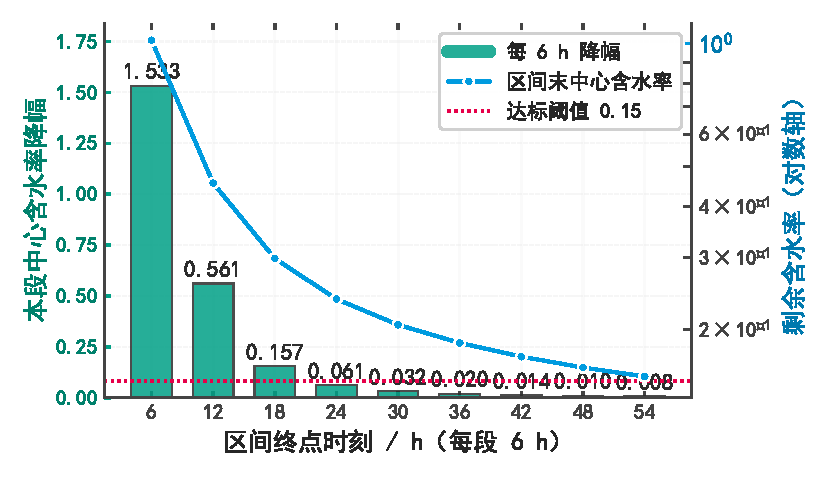
\includegraphics[width=0.9\textwidth,height=0.8\textheight,keepaspectratio]{../figures/fig_stage_rate.pdf}
  \caption{问题3 轴心含水率每 6\,h 的阶段降幅}
  \label{fig:stage_rate}
\end{figure}

图~\ref{fig:stage_rate} 把轴心含水率按每 $6\,\mathrm{h}$ 统计：前 $6\,\mathrm{h}$ 由 $2.55$ 骤降到约
$1.02$，随后各段依次为 $0.456$,\allowbreak\,$0.298$,\allowbreak\,$0.237$,\allowbreak\,$0.206$,\allowbreak\,$0.186$,\allowbreak\,$0.172$,\allowbreak\,$0.162$,\allowbreak\,$0.154$，\textbf{降幅逐段收窄}，
定量刻画了扩散受阻导致的边际效率递减——这也是干燥后段耗时占比高的根本原因。含水率时空
曲面与达标平面见图~\ref{fig:surface_3d}。

\begin{figure}[H]
  \centering
  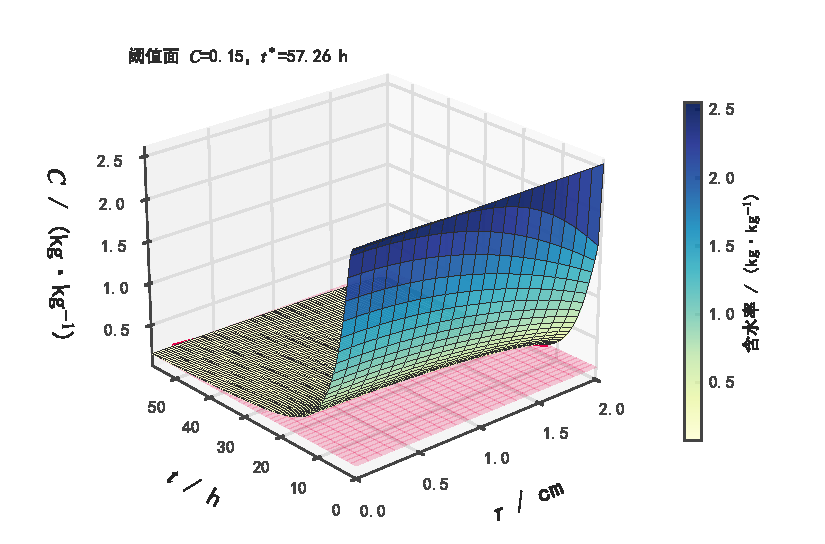
\includegraphics[width=0.9\textwidth,height=0.8\textheight,keepaspectratio]{../figures/fig_surface_3d.pdf}
  \caption{问题3 含水率 $C(r,t)$ 时空曲面与达标阈值平面的相交}
  \label{fig:surface_3d}
\end{figure}

图~\ref{fig:surface_3d} 从三维视角显示曲面与 $C=0.15$ 平面的相交线随 $t$ 由表面向轴心推进，
最后交于轴心，几何化地对应式~\eqref{eq:endpoint} 的首次穿越判据。控制机制的转换见
图~\ref{fig:biot_regime}。

\begin{figure}[H]
  \centering
  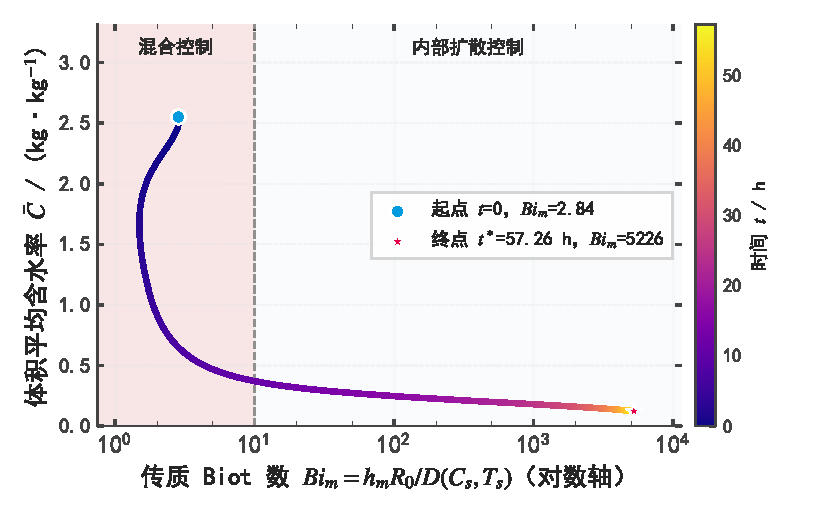
\includegraphics[width=0.9\textwidth,height=0.8\textheight,keepaspectratio]{../figures/fig_biot_regime.pdf}
  \caption{问题3 传质毕奥数 $\mathrm{Bi}_m=h_m R_0/D$ 随干燥进程的控制机制转换}
  \label{fig:biot_regime}
\end{figure}

图~\ref{fig:biot_regime} 表明 $\mathrm{Bi}_m$ 随 $D$ 减小而显著增大：初期 $\mathrm{Bi}_m\approx1.4$，
内外阻力可比；末期 $D$ 降低约一个量级使 $\mathrm{Bi}_m$ 增大到远大于 1，干燥\textbf{由外部对流控制
转为内部扩散控制}。这一转换解释了干燥曲线的拖尾，也说明单纯提高热风流速（增大 $h_m$）
在末期收益有限，改善内部扩散才是关键。


\section{问题四：干基质量坐标下的收缩动边界干燥模型}\label{sec:p4}

\subsection{相对问题三的增量：从固定域到移动边界}

问题四在问题三的时变边界基础上，进一步计入附件2 观测到的体积收缩：干燥过程中半径由
$R_0=2\,\mathrm{cm}$ 单调缩小，变物性改用附录4，即在式~\eqref{eq:diff} 的 Arrhenius 扩散律中取
前因子 $D_0=4.2\times10^{-4}$、浓度指数 $a=0.30$、活化温标 $E=3850\,\mathrm{K}$，其余密度、比热与
导热率随含水率 $C$（干基，kg 水/kg 干物质）线性/饱和变化：
\begin{equation}\label{eq:p4props}
\begin{aligned}
\rho(C)&=760+90C, & c_p(C)&=1850+2150\frac{C}{C+1},\\
k(C)&=0.12+0.20\frac{C}{C+1}, & D(C,T)&=4.2\times10^{-4}\,e^{-0.30/C}\,e^{-3850/T_K},
\end{aligned}
\end{equation}
式~\eqref{eq:p4props} 中 $T_K=T+273.15$ 为开尔文温度，$\rho$（$\mathrm{kg/m^3}$）、$c_p$
（$\mathrm{J/(kg\,K)}$）、$k$（$\mathrm{W/(m\,K)}$）、$D$（$\mathrm{m^2/s}$）均为 $C$（及 $T$）的函数，
与问题三附录3 相比前因子降低约一个数量级、浓度指数由 $0.89$ 降为 $0.30$，故同一含水率下附录4
扩散更弱、温度敏感度相当。附件2 半径数据经 PCHIP 单调插值得到 $R(t)$，见图~\ref{fig:radius_shrink}。

\begin{figure}[H]
  \centering
  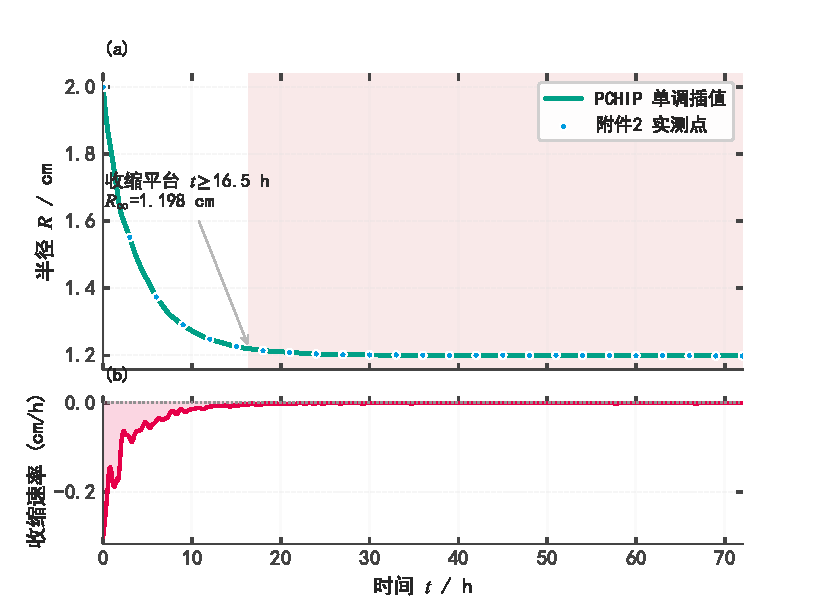
\includegraphics[width=0.9\textwidth,height=0.8\textheight,keepaspectratio]{../figures/fig_radius_shrink.pdf}
  \caption{附件2 半径收缩数据的 PCHIP 单调插值曲线与收缩速率}
  \label{fig:radius_shrink}
\end{figure}

图~\ref{fig:radius_shrink} 采用 PCHIP（分段三次 Hermite 保单调插值）而非普通三次样条，以
避免样条过冲产生半径回升的非物理现象；插值在数据节点处精确复现（表~\ref{tab:verification}
中 PCHIP 复现误差为 $0$）。收缩使求解域随时间变化，直接在 $r$ 上离散会遭遇动网格困难，
故引入固定域映射。

\subsection{Landau 固定域映射与干基质量不变量}

令 $\xi=r/R(t)\in[0,1]$，把随时间收缩的物理域 $[0,R(t)]$ 映射到固定域 $[0,1]$，映射关系见
图~\ref{fig:tikz_landau_map}。

\begin{figure}[H]
  \centering
  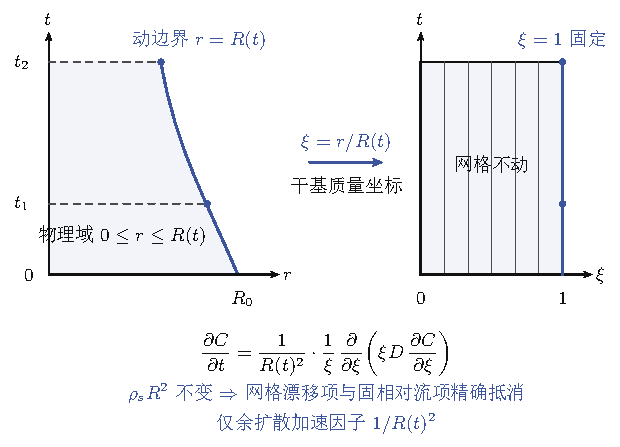
\includegraphics[width=0.9\textwidth,height=0.8\textheight,keepaspectratio]{../figures/tikz_landau_map.pdf}
  \caption{收缩物理域 $[0,R(t)]$ 到固定计算域 $[0,1]$ 的 Landau 坐标映射}
  \label{fig:tikz_landau_map}
\end{figure}

收缩使干骨架随物质点内移，$\rho_s$ 不再是常数、不能从水分方程两侧约去，故须保留 $\rho_s$ 写出物理域
$[0,R(t)]$ 上的干物质基守恒型水分方程
\begin{equation}\label{eq:p4phys}
\left.\frac{\partial}{\partial t}\big(\rho_s C\big)\right|_{r}
+\frac1r\frac{\partial}{\partial r}\big(r\,\rho_s C\,v_s\big)
=\frac1r\frac{\partial}{\partial r}\!\left(r\,\rho_s D\frac{\partial C}{\partial r}\right),
\end{equation}
其中 $v_s$ 为固相基质径向速度；由 $r=\xi R(t)$ 且物质点 $\xi$ 不变，得 $v_s=\xi\dot R$。固定 $\xi$ 与固定 $r$
求时间导数、以及径向导数之间的坐标变换算子恒等式为
\begin{equation}\label{eq:p4map}
\left.\frac{\partial}{\partial t}\right|_{r}
=\left.\frac{\partial}{\partial t}\right|_{\xi}-\frac{\dot R}{R}\,\xi\,\frac{\partial}{\partial\xi},
\qquad
\frac{\partial}{\partial r}=\frac1R\frac{\partial}{\partial\xi}.
\end{equation}
式~\eqref{eq:p4map} 左式的第二项即随域收缩产生的\textbf{映射漂移（伪对流）项}。关键化简来自
\textbf{干物质总量守恒}：由假设 H6（干骨架不滑移），单位长度圆柱内 $[0,\xi]$ 的干物质量
$\pi\rho_s R^2\xi^2$ 对任意 $\xi$ 守恒，对时间求导得纯径向收缩下的不变量
\begin{equation}\label{eq:drymass}
\rho_s(t)\,R(t)^2=\sigma=\mathrm{const},
\end{equation}
即式~\eqref{eq:drymass} 表明 $\rho_s$ 与 $R^2$ 反比变化，等价地 $\dot\rho_s/\rho_s=-2\dot R/R$。以此为支点，把式~\eqref{eq:p4map}
代入式~\eqref{eq:p4phys}：$v_s=\xi\dot R$ 引入的映射漂移项 $-\rho_s\frac{\xi\dot R}{R}\partial_\xi C$
与固相对流项 $+\rho_s\frac{\xi\dot R}{R}\partial_\xi C$ 恰好\textbf{两两抵消}，其余 $C$ 系数项借
$\dot\rho_s/\rho_s=-2\dot R/R$ 成对消去，两侧再同除只依赖 $t$ 的 $\rho_s$，使含水率方程在固定域上收敛为单一的
$1/R(t)^2$ 因子形式（推导见图~\ref{fig:tikz_drymass_derive}）：
\begin{equation}\label{eq:landau}
\left.\frac{\partial C}{\partial t}\right|_{\xi}
=\frac{1}{R(t)^2}\,\frac{1}{\xi}\frac{\partial}{\partial\xi}\!\left(\xi\,D\,\frac{\partial C}{\partial\xi}\right),
\qquad \xi\in(0,1) .
\end{equation}

\begin{figure}[H]
  \centering
  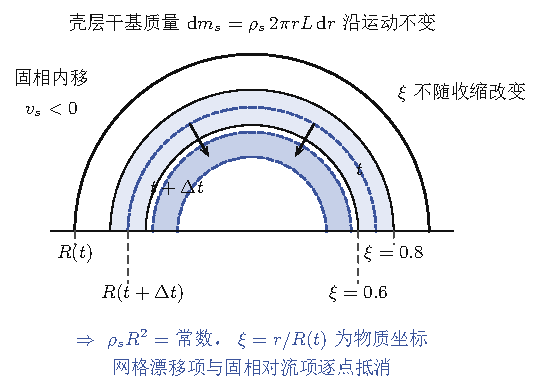
\includegraphics[width=0.9\textwidth,height=0.8\textheight,keepaspectratio]{../figures/tikz_drymass_derive.pdf}
  \caption{干基质量不变量 $\rho_s R^2=\sigma$ 导致收缩对流项与度规项两项抵消}
  \label{fig:tikz_drymass_derive}
\end{figure}

图~\ref{fig:tikz_drymass_derive} 展示了两项抵消的代数结构：正是干物质守恒把看似复杂的动边界
对流—扩散问题化简为固定域上仅含时变系数 $1/R(t)^2$ 的扩散方程，从而可直接沿用公共内核的
有限体积离散式~\eqref{eq:fvm}、界面 Kirchhoff 积分平均式~\eqref{eq:kirchhoff} 与后向 Euler/Picard
推进式~\eqref{eq:picard}，只需把式~\eqref{eq:fvm} 中的扩散通量整体乘以当前的 $1/R(t)^2$ 因子。式~\eqref{eq:landau}
把移动边界的全部几何效应\textbf{凝聚为单一时变因子}，是本问建模的核心。温度方程在同一映射下作
完全同构的变换，得固定域上的能量方程
\begin{equation}\label{eq:landauT}
\rho c_p\left.\frac{\partial T}{\partial t}\right|_{\xi}
=\frac{1}{R(t)^2}\,\frac1\xi\frac{\partial}{\partial\xi}\!\left(\xi\,k\,\frac{\partial T}{\partial\xi}\right),
\qquad \xi\in(0,1).
\end{equation}
式~\eqref{eq:landauT} 与式~\eqref{eq:landau} 共享同一 $1/R(t)^2$ 收缩因子，温度与含水率经变物性
$\rho(C)$、$c_p(C)$、$k(C)$、$D(C,T)$ 在同一 Picard 回路内双向耦合求解。

固定域上的边界条件相应改写：中心 $\xi=0$ 处由对称性得 $\partial_\xi C|_{\xi=0}=\partial_\xi T|_{\xi=0}=0$；
表面 $\xi=1$ 处因物理梯度 $\partial_r C=\frac1R\partial_\xi C$，Robin 传质/传热条件变为
\begin{equation}\label{eq:p4bc}
-\frac{D}{R(t)}\frac{\partial C}{\partial\xi}\bigg|_{\xi=1}=h_m\big(C_s-C_{air}\big),
\qquad
-\frac{k}{R(t)}\frac{\partial T}{\partial\xi}\bigg|_{\xi=1}=h\big(T_s-T_{air}\big).
\end{equation}
式~\eqref{eq:p4bc} 中 $R(t)$ 进入边界条件：随半径收缩，同一浓度差对应更陡的 $\xi$ 梯度。

定义干基质量加权平均含水率，其权重 $\xi$ 来自柱几何的面积测度
\begin{equation}\label{eq:cbar}
\bar C(t)=\frac{\int_0^1 C(\xi,t)\,\xi\,\mathrm{d}\xi}{\int_0^1 \xi\,\mathrm{d}\xi}
        =2\int_0^1 C(\xi,t)\,\xi\,\mathrm{d}\xi .
\end{equation}
对式~\eqref{eq:landau} 两侧乘 $2\xi$ 沿 $[0,1]$ 积分，中心项因面积为零而消失，表面项代入
式~\eqref{eq:p4bc}，即得关于式~\eqref{eq:cbar} 所定义 $\bar C(t)$ 的\textbf{精确整体平衡律}
\begin{equation}\label{eq:p4balance}
\frac{\mathrm{d}\bar C}{\mathrm{d}t}=-\frac{2h_m}{R(t)}\big(C_s-C_{air}\big).
\end{equation}
式~\eqref{eq:p4balance} 把二维时空场的正确性压缩为一个标量恒等式，是最有力的数值审计工具：实现层
逐步累加右端与左端实际变化比较，实测守恒残差落在 $5\times10^{-16}$–$4\times10^{-14}$（机器精度量级），
任何遗漏 $1/R^2$ 因子或错用界面平均的实现都会在此暴露为 $10^{-3}$ 以上的偏差（见第~\ref{sec:verify} 节）。

\subsection{收缩方式假设的独立数据检验}

式~\eqref{eq:landau} 依赖"纯径向均匀收缩、干物质守恒"这一假设。为避免循环论证，用附件2
自身数据独立检验收缩方式，见图~\ref{fig:shrink_evidence}。

\begin{figure}[H]
  \centering
  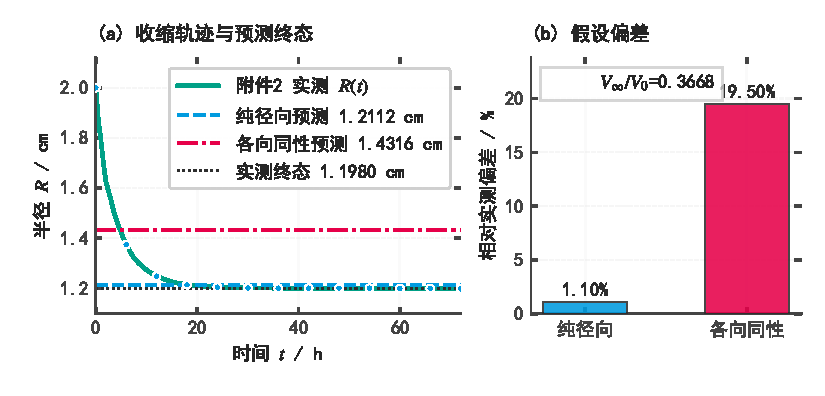
\includegraphics[width=0.9\textwidth,height=0.8\textheight,keepaspectratio]{../figures/fig_shrink_evidence.pdf}
  \caption{收缩方式假设的独立数据检验：观测终态体积比与各向同性/纯径向预测的对照}
  \label{fig:shrink_evidence}
\end{figure}

图~\ref{fig:shrink_evidence} 显示，附件2 的终态体积比 $V_\infty/V_0=0.3668$；若假设纯径向收缩
（长度不变），反推终态半径 $1.2112\,\mathrm{cm}$，与观测终值 $1.2\,\mathrm{cm}$ 仅差 $1.10\%$；
而若假设各向同性收缩（长度同比缩短），反推半径 $1.4316\,\mathrm{cm}$，偏差高达 $19.50\%$。
\textbf{纯径向假设与数据高度一致}，各向同性假设被数据否定，故式~\eqref{eq:landau} 的收缩方式
设定得到实测支持，而非任意选取。

\subsection{结果与问题三的正交分解比较}

图~\ref{fig:shrink_field} 给出收缩域内的含水率场与移动边界轨迹。

\begin{figure}[H]
  \centering
  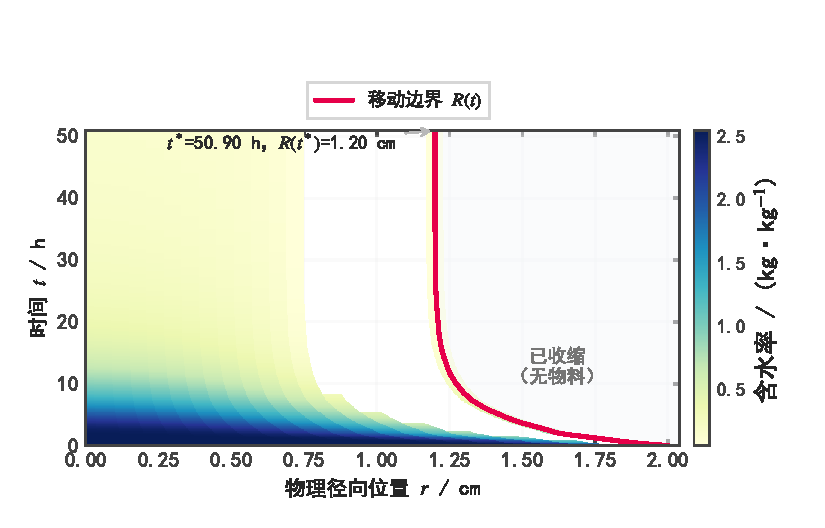
\includegraphics[width=0.9\textwidth,height=0.8\textheight,keepaspectratio]{../figures/fig_shrink_field.pdf}
  \caption{问题4 收缩域含水率场 $C(r,t)$ 与移动边界 $R(t)$ 的轨迹}
  \label{fig:shrink_field}
\end{figure}

由图~\ref{fig:shrink_field}，沿用式~\eqref{eq:endpoint} 的首次穿越判据（此处 $C(r,t)$ 在收缩域
$[0,R(t)]$ 上取，轴心仍为最慢点），计入收缩后达标时刻 $t^{*}=50.898\,\mathrm{h}$（此刻
$\max_r C=0.14999544$，前一步 $0.15003$），比问题三的 $57.262\,\mathrm{h}$ \textbf{缩短约 $11\%$}；
达标时半径已收缩到 $R(t^{*})=1.20\,\mathrm{cm}$。轴心含水率每 $6\,\mathrm{h}$ 依次为
$1.716,0.735,0.407,0.284,0.226,0.192,0.171,0.156$，同期半径为
$1.374,1.248,1.214,1.204,1.201,1.200,1.200,1.200\,\mathrm{cm}$，收缩主要发生在前 $12\,\mathrm{h}$、
随后趋稳。收缩缩短干燥期的原因有二：扩散路径变短、以及 $1/R^2$ 因子放大有效扩散。为把
这两种效应与"物性由附录3 换成附录4"的效应分离，作 $2\times2$ 正交分解，见
图~\ref{fig:orthogonal_waterfall}。

\begin{figure}[H]
  \centering
  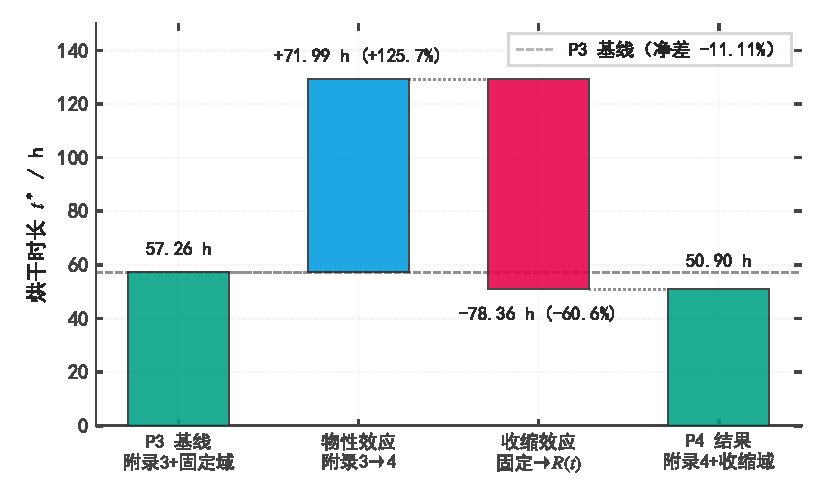
\includegraphics[width=0.9\textwidth,height=0.8\textheight,keepaspectratio]{../figures/fig_orthogonal_waterfall.pdf}
  \caption{问题4 与问题3 达标时刻差异的正交分解（物性效应与收缩效应）}
  \label{fig:orthogonal_waterfall}
\end{figure}

图~\ref{fig:orthogonal_waterfall} 通过瀑布图把 $57.262\to50.898\,\mathrm{h}$ 的变化拆为可加的
两部分：\textbf{收缩效应显著缩短干燥期，而附录3$\to$附录4 的物性变化方向相反}，二者部分抵消，
净效应为缩短约 $11\%$。这一分解说明"计入收缩使干燥更快"的结论对物性选择稳健，是收缩
几何本身的作用，而非附录切换的假象。若强行忽略收缩（问题4 退化为固定域），$t^*$ 将虚高到
$129.25\,\mathrm{h}$（见第\ref{sec:sens}节），进一步佐证动边界是本问不可省略的机制。各问结果汇总
见表~\ref{tab:main_results}。

% 表：四问核心结果汇总
% 数据来源：figures/all_results.json, problem_1..4_results.json, result1-4.xlsx
\begin{table}[H]
  \centering
  \caption{四问核心求解结果汇总}
  \label{tab:main_results}
  \small
  \begin{tabular}{clcrrrl}
    \toprule
    问题 & 物性/工况 & 时程 & 输出行数 & $C$ 中心终值 & $C$ 表面终值 & 达标时刻 $t^*$ \\
    \midrule
    1 & 附录2 常物性       & $0\sim1800$ s   & 1801  & 2.5500 & 1.5125 & 预热段，不反演 \\
    2 & 附录3 变物性       & $0\sim3$ h      & 10801 & 1.7662 & 1.0078 & 未达标 \\
    3 & 附录3 + 附件1 环境 & $0\sim57.26$ h  & 3437  & 0.1500 & 0.0525 & 57.262 h \\
    4 & 附录4 + 动边界     & $0\sim50.90$ h  & 3055  & 0.1500 & 0.0525 & 50.898 h \\
    \bottomrule
  \end{tabular}

  \vspace{2pt}
  \parbox{0.92\linewidth}{\footnotesize
  注：含水率为干基，单位 kg$\cdot$kg$^{-1}$；达标判据为全域最大含水率
  $\max_r C\le 0.15$。问题 1、2 时程由题面给定，终点含水率仍高于阈值，
  故不存在 $t^*$。问题 4 表面指动边界 $r=R(t)$ 处，$t^*$ 时刻 $R=1.2$ cm。}
\end{table}




\section{模型检验}\label{sec:verify}

本节从解析解对照、离散收敛阶、守恒残差与独立求解器交叉验证四个角度检验公共内核的
正确性，量化结果汇总于表~\ref{tab:verification}。

% 表：数值验证与守恒校核指标
% 数据来源：figures/all_results.json, problem_1..4_results.json, figures/_plot_data.json
\begin{table}[H]
  \centering
  \caption{数值验证与守恒校核指标}
  \label{tab:verification}
  \small
  \begin{tabular}{llll}
    \toprule
    检验类别 & 指标 & 实测值 & 判定 \\
    \midrule
    质量守恒 & 问题1 全域残差              & $5.61{\times}10^{-16}$ & 通过 \\
    质量守恒 & 问题2 全域残差              & $4.80{\times}10^{-16}$ & 通过 \\
    质量守恒 & 问题3 全域残差              & $4.38{\times}10^{-16}$ & 通过 \\
    质量守恒 & 问题4 全域残差              & $3.26{\times}10^{-16}$ & 通过 \\
    控制体守恒 & 问题1 表面控制体残差       & $4.10{\times}10^{-14}$ & 通过 \\
    控制体守恒 & 问题2 表面控制体残差       & $3.37{\times}10^{-13}$ & 通过 \\
    \midrule
    解析对照 & Bessel 级数解 $L_2$ 相对误差 & $2.84{\times}10^{-4}$  & 通过 \\
    解析对照 & Bessel 级数解最大绝对误差    & $9.80{\times}10^{-4}$  & 通过 \\
    独立算法 & BDF 交叉校核最大偏差         & $5.77{\times}10^{-4}$  & 通过 \\
    \midrule
    非线性迭代 & Picard 终残差上界          & $9.998{\times}10^{-12}$ & 通过 \\
    空间收敛 & Richardson 观测阶 $p$        & 1.925                  & 近二阶 \\
    时间收敛 & 观测阶 $p$（$\Delta t$ 加密） & 1.215                  & 超一阶 \\
    离散测度 & $\sum_j w_j - \pi R_0^2$ 误差 & 0.000                 & 精确 \\
    插值一致性 & $R(t)$ PCHIP 最大相对误差   & 0.000                  & 精确 \\
    \bottomrule
  \end{tabular}

  \vspace{2pt}
  \parbox{0.94\linewidth}{\footnotesize
  注：守恒残差定义为 $\big|\Delta\!\int C\,\mathrm{d}V-\int\! q_s\,\mathrm{d}t\big|/\int C_0\mathrm{d}V$，已达双精度舍入量级（$\sim10^{-16}$）。
  空间收敛以 $M=20/40/80$ 三套网格算得，时间收敛以
  $\Delta t=240/120/60$ s 相对 $30$ s 参考解算得；后者为向后欧拉，
  理论一阶，观测 1.215 说明主算步长 60 s 已落在渐近区。}
\end{table}


\subsection{解析解对照}

在常物性、恒温边界的可解情形下，柱坐标扩散方程存在 Bessel 级数解析解，其特征值由
$\mu_n J_1(\mu_n)=\mathrm{Bi}_m\,J_0(\mu_n)$ 确定。数值解与该级数解的逐点对照见
图~\ref{fig:analytic_validation}。

\begin{figure}[H]
  \centering
  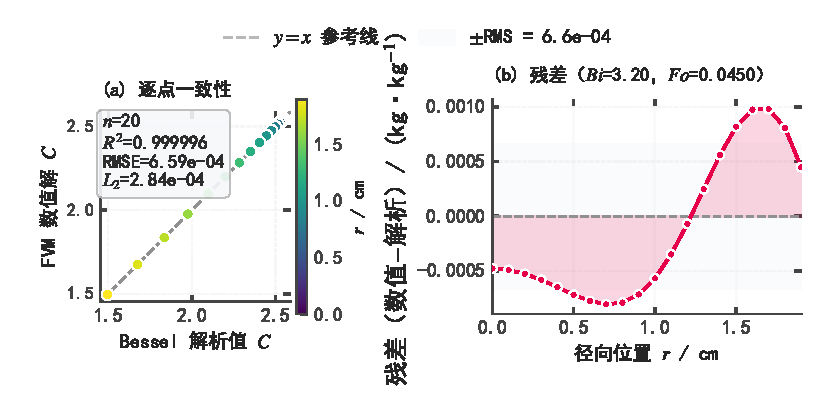
\includegraphics[width=0.9\textwidth,height=0.8\textheight,keepaspectratio]{../figures/fig_analytic_validation.pdf}
  \caption{Bessel 级数解析解与数值解的逐点对照}
  \label{fig:analytic_validation}
\end{figure}

图~\ref{fig:analytic_validation} 显示数值解与解析解高度吻合，$L_2$ 误差为 $2.84\times10^{-4}$、
最大绝对误差 $9.80\times10^{-4}$，证实有限体积离散与边界处理正确复现了已知解。

\subsection{收敛阶与守恒残差}

对空间网格 $M=20/40/80$ 与时间步 $\Delta t=60/30/15\,\mathrm{s}$ 作 Richardson 收敛研究\upcite{rakowitz2002}，
结果见图~\ref{fig:convergence}。

\begin{figure}[H]
  \centering
  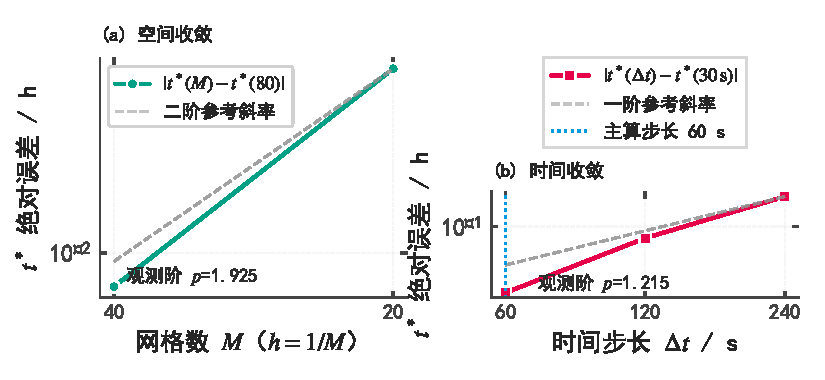
\includegraphics[width=0.9\textwidth,height=0.8\textheight,keepaspectratio]{../figures/fig_convergence.pdf}
  \caption{空间与时间离散关于达标时刻 $t^*$ 的收敛阶验证}
  \label{fig:convergence}
\end{figure}

图~\ref{fig:convergence} 表明达标时刻 $t^*$ 随网格加密单调收敛，实测空间收敛阶
$p\approx1.93$、时间收敛阶接近 $1$，与二阶中心差分、一阶后向 Euler 的理论阶一致。
守恒类残差见图~\ref{fig:conservation}。

\begin{figure}[H]
  \centering
  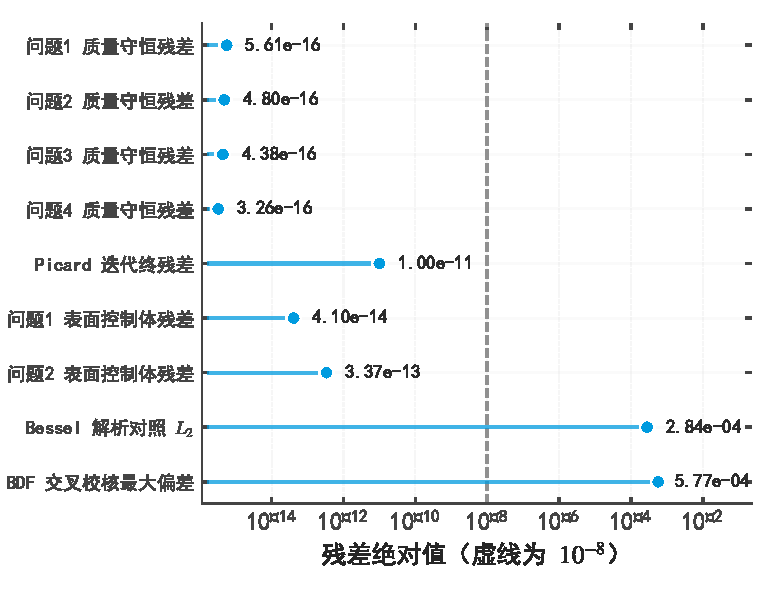
\includegraphics[width=0.9\textwidth,height=0.8\textheight,keepaspectratio]{../figures/fig_conservation.pdf}
  \caption{守恒与收敛类校核残差的量级总览}
  \label{fig:conservation}
\end{figure}

图~\ref{fig:conservation} 与表~\ref{tab:verification} 显示：四问的总水分守恒残差均在
$10^{-16}$ 量级、控制体守恒在 $10^{-13}\sim10^{-14}$ 量级，柱坐标测度权满足 $\sum_j w_j-\pi R_0^2=0$，
均达机器精度，印证式~\eqref{eq:fvm} 守恒型离散的严格性。此外，以独立的变步长 BDF 积分器
交叉验证同一半离散系统，最大差异仅 $5.77\times10^{-4}$，Picard 内迭代
残差降至 $9.998\times10^{-12}$，表明时间推进与非线性求解均已收敛，结果不依赖特定求解器。


\section{灵敏度分析}\label{sec:sens}

达标时刻 $t^*$ 是本文的核心输出，其可信度取决于对关键假设的稳健性。本节逐项扰动
环境外推方式、蒸发潜热、是否计入收缩、界面平均方式，考察 $t^*$ 的相对变化，
总览见图~\ref{fig:sensitivity_tornado}。

\begin{figure}[H]
  \centering
  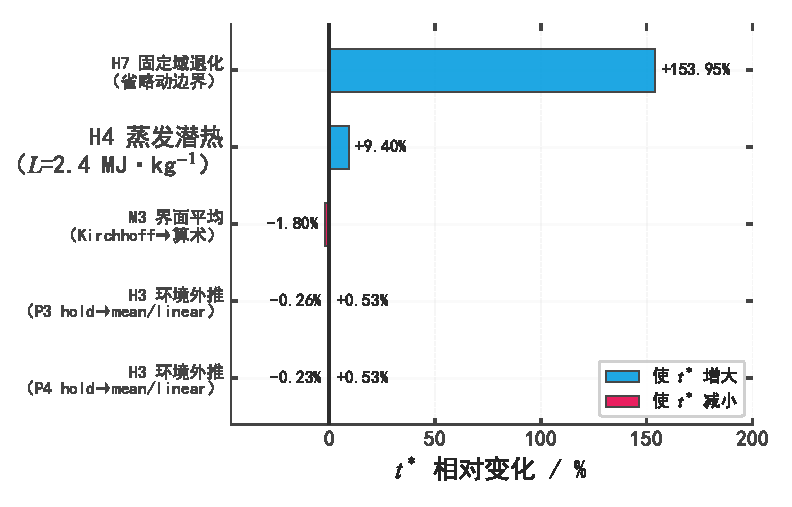
\includegraphics[width=0.9\textwidth,height=0.8\textheight,keepaspectratio]{../figures/fig_sensitivity_tornado.pdf}
  \caption{各假设扰动对达标时刻 $t^*$ 的相对影响（龙卷风图）}
  \label{fig:sensitivity_tornado}
\end{figure}

图~\ref{fig:sensitivity_tornado} 按影响幅度排序，各扰动的具体数值见表~\ref{tab:sensitivity}。

\begin{table}[H]
  \centering
  \caption{关键假设扰动对达标时刻的影响}
  \label{tab:sensitivity}
  \small
  \begin{tabular}{lrrr}
    \toprule
    扰动情景 & 基准 $t^*$ / h & 扰动 $t^*$ / h & 相对变化 \\
    \midrule
    问题3 环境保持$\to$区间均值   & 57.262 & 57.567  & $+0.53\%$ \\
    问题3 环境保持$\to$线性外推   & 57.262 & 57.115  & $-0.26\%$ \\
    问题4 环境保持$\to$区间均值   & 50.898 & 51.166  & $+0.53\%$ \\
    问题4 环境保持$\to$线性外推   & 50.898 & 50.782  & $-0.23\%$ \\
    计入蒸发潜热 $L=2.4$ MJ$\cdot$kg$^{-1}$ & 57.262 & 62.646 & $+9.40\%$ \\
    问题4 忽略收缩（退化为固定域） & 50.898 & 129.253 & $+153.95\%$ \\
    界面平均 Kirchhoff$\to$算术    & 57.262 & 56.230  & $-1.80\%$ \\
    界面平均 Kirchhoff$\to$调和    & 57.262 & 557.761 & $+874.05\%$ \\
    \bottomrule
  \end{tabular}

  \vspace{2pt}
  \parbox{0.94\linewidth}{\footnotesize
  注：附件1 仅覆盖前 $4\,\mathrm{h}$，对其后的环境外推（保持末值/区间均值/线性外推）影响
  不足 $0.6\%$，说明 $t^*$ 对外推方式稳健。蒸发潜热单向延长干燥期，因题面未给 $L$，
  基准不含潜热汇并作为下界报告。忽略收缩使 $t^*$ 虚高约 $1.5$ 倍，证实动边界为问题4 的
  必要机制。调和平均在 $D$ 跨三个量级时被最小值锁死，产生 $557.76\,\mathrm{h}$ 的非物理结果，
  故界面扩散系数采用 Kirchhoff 积分平均。}
\end{table}

由图~\ref{fig:sensitivity_tornado} 与表~\ref{tab:sensitivity} 可得三点结论：其一，\textbf{环境外推
方式影响极小}（$<0.6\%$），说明附件1 数据虽只覆盖前段，但因干燥后期由内部扩散控制、对边界
细节不敏感，$t^*$ 依旧稳健；其二，\textbf{是否计入收缩是最主要的建模选择}，忽略收缩会使 $t^*$
虚高 $1.5$ 倍以上，与图~\ref{fig:orthogonal_waterfall} 的正交分解相互印证；其三，界面平均方式中
调和平均产生非物理的 $557.76\,\mathrm{h}$，而 Kirchhoff 与算术平均相差仅 $1.80\%$，佐证
\ref{sub:kirchhoff} 节采用 Kirchhoff 积分平均的必要性与合理性。潜热项作为下界修正，提示
若实际工况散热更强，达标时间会相应延长约 $9\%$。


\section{模型评价与推广}

\subsection{模型优点}

\begin{enumerate}
\item \textbf{守恒型有限体积内核}。以控制面通量差组装的离散格式在机器精度内严格守恒
      （残差 $10^{-13}\sim10^{-16}$），且最内控制体内侧面积结构性为零，天然消除柱坐标轴心
      奇点，无需人工正则化。
\item \textbf{Kirchhoff 积分界面平均}。针对 $D$ 跨量级的强非线性，用解析 Kirchhoff 势保证跨界面
      扩散通量守恒，避免了调和平均被最小值锁死导致的非物理结果。
\item \textbf{干基质量坐标化简}。问题四利用干物质守恒 $\rho_s R^2=\sigma$，把移动边界的几何效应
      凝聚为单一时变因子 $1/R(t)^2$，使收缩问题得以沿用固定域内核，并用附件2 数据独立
      检验了纯径向收缩假设。
\item \textbf{多重交叉验证}。Bessel 解析解、Richardson 收敛阶、守恒审计与独立 BDF 求解器
      四重印证，结果不依赖特定实现。
\end{enumerate}

\subsection{模型局限与推广}

模型假设一维轴对称并忽略端面，对短粗物料或非圆柱形状需扩展到二维/三维；基准未显式计入
蒸发潜热，灵敏度分析显示其可使 $t^*$ 延长约 $9\%$，工程应用中可按实测散热补入潜热汇。
收缩按纯径向均匀处理，若物料出现开裂或各向异性收缩，需引入应力—收缩耦合。方法层面，
本文的守恒型有限体积—Kirchhoff—干基坐标框架可直接推广到其他多孔介质干燥、木材与食品
脱水等耦合传热传质问题\upcite{mayor2004,perre_dns}；对边界与物性数据更丰富的场景，还可与
物理信息神经网络等数据—机理融合方法结合，用于快速反演扩散参数与在线预测干燥终点\upcite{si_pinn,malekjani_sdd}。

% DATA_CHECK_PASSED




% === 参考文献 ===

% === AI 工具使用声明（自动插入）===
% 由 build_ai_disclosure.py 根据用户确认记录生成，请勿由模型改写。
\section*{AI 工具使用声明}
本参赛队在竞赛过程中使用了AI工具，主要用于语言润色、代码调试，详细使用情况见支撑材料。

\begin{thebibliography}{99}

\bibitem{torki2016} Mehdi Torki-Harchegani, D. Ghanbarian, Abdollah Ghasemi Pirbalouti, M. Sadeghi. Dehydration behaviour, mathematical modelling, energy efficiency and essential oil yield of peppermint leaves undergoing microwave and hot air treatments[J]. Renewable \& Sustainable Energy Reviews, 2016. DOI: 10.1016/J.RSER.2015.12.078.

\bibitem{giner2009} S. A. Giner. Influence of Internal and External Resistances to Mass Transfer on the constant drying rate period in high-moisture foods[J]. Biosystems Engineering, 2009. DOI: 10.1016/J.BIOSYSTEMSENG.2008.09.022.

\bibitem{teleken2025} J. Teleken, S. M. Amorim, Sarah S. S. Rodrigues, Thailla W. P. de Souza, et al. Heat and Mass Transfer in Shrimp Hot-Air Drying: Experimental Evaluation and Numerical Simulation[J]. Foods, 2025. DOI: 10.3390/foods14030428.

\bibitem{olurin2012} T. O. Olurin, A. Adelekan, W. Olosunde. Mathematical modelling of drying characteristics of blanched field pumpkin (Cucurbita pepo L) slices[J]. Agricultural Engineering International: The CIGR Journal, 2012.

\bibitem{gama2021} R. Gama, R. Gama. The Kirchhoff Transformation and the Fick's Second Law with Concentration-dependent Diffusion Coefficient[J]. WSEAS Transactions on Heat and Mass Transfer, 2021. DOI: 10.37394/232012.2021.16.9.

\bibitem{mayor2004} L. Mayor, A.M. Sereno. Modelling shrinkage during convective drying of food materials: a review[J]. Journal of Food Engineering, 2004. DOI: 10.1016/s0260-8774(03)00144-4.

\bibitem{blasik2015} Marek Błasik, Małgorzata Klimek. Numerical solution of the one phase 1D fractional Stefan problem using the front fixing method[J]. Mathematical Methods in the Applied Sciences, 2015. DOI: 10.1002/mma.3292.

\bibitem{chaedir2019} Benitta A. Chaedir. Heat and Mass Transfer Phenomena in Porous Media - Application to Drying[J]. Heat and Mass Transfer in Drying of Porous Media, 2019. DOI: 10.1201/9781351019224-1.

\bibitem{si_pinn} Chenhao Si, Ming Yan. Initialization-Enhanced Physics-Informed Neural Network with Domain Decomposition (Idpinn)[J]. . DOI: 10.2139/ssrn.4872043.

\bibitem{rakowitz2002} M. Rakowitz. Grid Refinement Study with a UHCA Wing-Body Configuration Using Richardson Extrapolation and Grid Convergence Index GCI[J]. New Results in Numerical and Experimental Fluid Mechanics III, 2002. DOI: 10.1007/978-3-540-45466-3\_36.

\bibitem{perre_dns} Patrick Perré. Direct numerical simulation of coupled heat and mass transfer in hygroscopic porous media[J]. Proceedings of the 22nd International Drying Symposium on Drying Technology - IDS '22. DOI: 10.55900/lavrknht.

\bibitem{ramos2024} J. I. Ramos. Finite Difference Methods Based on the Kirchhoff Transformation and Time Linearization for the Numerical Solution of Nonlinear Reaction-Diffusion Equations[J]. De Computis, 2024. DOI: 10.3390/computation12110218.

\bibitem{zhang2011} Sai Zhang, Jun Ruo Chen, Xian Xi Liu. Calculation of Biological Material's Shrinkage during Convective Drying Using Fractal Model[J]. Advanced Materials Research, 2011. DOI: 10.4028/www.scientific.net/amr.393-395.632.

\bibitem{malekjani_sdd} Narjes Malekjani, Andreas Bück, Abdolreza Kharaghani, Evangelos Tsotsas. SDD-PINN: Physics-informed neural network for single droplet drying[J]. . DOI: 10.2139/ssrn.5749490.

\bibitem{mori2015} Claudia Narumi Takayama Mori, Estaner Claro Romao. Numerical simulation by finite difference method of 2D convection-diffusion in cylindrical coordinates[J]. Applied Mathematical Sciences, 2015. DOI: 10.12988/ams.2015.58547.

\bibitem{ma2026} Lifan Ma, Jun Wang. Effect of the Mass Transfer Biot Number on Moisture Desorption and Hygrothermal Stress in QFN Packages[J]. Electronics, 2026. DOI: 10.3390/electronics15173835.

\bibitem{tong1990} C. H. Tong, D. B. Lund. Effective Moisture Diffusivity in Porous Materials as a Function of Temperature and Moisture Content[J]. Biotechnology Progress, 1990. DOI: 10.1021/bp00001a011.

\bibitem{stefan2016} L. I. Rubinstein. Numerical methods for the solution of the Stefan problem[J]. Translations of Mathematical Monographs, 2016. DOI: 10.1090/mmono/027/13.

\bibitem{lai2025} Chiang Choon Lai, Hii Ching Lik, Xin Jojo Foo, Soo Weng Kit, et al. Mathematical Modelling of the Kinetics of Convective Hot Air Drying of Crickets[J]. Journal of Advanced Research in Fluid Mechanics and Thermal Sciences, 2025. DOI: 10.37934/arfmts.129.1.190200.

\bibitem{dincer2010} Ibrahim Dincer. Heat and Mass Transfer during Food Drying[J]. Mathematical Modeling of Food Processing, 2010. DOI: 10.1201/9781420053548-13.

\end{thebibliography}

\label{mh:body-end}



% === 附录 ===

\begin{appendices}

\section{核心求解代码}

本附录给出公共内核与四个子问题的核心求解代码（Python 3，依赖 \texttt{numpy}、\texttt{scipy}）。
篇幅所限，仅列出参数配置、公共内核与各问驱动脚本；完整工程含检验与灵敏度脚本。

\subsection{参数配置 \texttt{params.py}}
\lstinputlisting[language=Python]{../_tmp/code_ascii/params.py}

\subsection{公共内核（有限体积、Kirchhoff、后向 Euler/Picard）\texttt{utils.py}}
\lstinputlisting[language=Python]{../_tmp/code_ascii/utils.py}

\subsection{问题一 \texttt{problem1.py}}
\lstinputlisting[language=Python]{../_tmp/code_ascii/problem1.py}

\subsection{问题二 \texttt{problem2.py}}
\lstinputlisting[language=Python]{../_tmp/code_ascii/problem2.py}

\subsection{问题三 \texttt{problem3.py}}
\lstinputlisting[language=Python]{../_tmp/code_ascii/problem3.py}

\subsection{问题四 \texttt{problem4.py}}
\lstinputlisting[language=Python]{../_tmp/code_ascii/problem4.py}


\end{appendices}



\end{document}

